%%%%%%%%%%%%%%%%%%%%%%%%%%%%%%%%%%%%%%%%%
% Short Sectioned Assignment LaTeX Template Version 1.0 (5/5/12)
% This template has been downloaded from: http://www.LaTeXTemplates.com
% Original author:  Frits Wenneker (http://www.howtotex.com)
% License: CC BY-NC-SA 3.0 (http://creativecommons.org/licenses/by-nc-sa/3.0/)
%%%%%%%%%%%%%%%%%%%%%%%%%%%%%%%%%%%%%%%%%

\documentclass[12pt, a4paper, oneside]{book}

\usepackage[utf8]{inputenc}             % Document encoding
\usepackage[T1]{fontenc}                % Use 8-bit encoding that has 256 glyphs
\usepackage[english]{babel}             % Support English
\usepackage{fourier}                    % Adobe Utopia font for the document
\usepackage{listings}                   % Code formatting
\usepackage{url}                        % URLs and hyperlinks
\usepackage{graphics, graphicx, float}  % Image positioning
\usepackage{cite}                       % Include cites from the bibliography.bib file
\usepackage{fancyhdr}                   % Custom headers and footers
\usepackage{enumitem}                   % For compact itemize
\usepackage{hyperref}
\usepackage{graphicx}
\usepackage{adjustbox}
\usepackage{geometry}
\usepackage{tabularx}
\usepackage{booktabs}
\usepackage{titlesec, blindtext, color}
\usepackage[Lenny]{fncychap}
\usepackage[table,xcdraw,x11names]{xcolor}
\usepackage[most]{tcolorbox}
\usepackage[style=indexgroup]{glossaries}
\usepackage{etoolbox}                   % For patching commands
\usepackage{tikz}
\usepackage{dirtree}
\usepackage{array}

\hypersetup{
	colorlinks=true,	  % False: boxed links; true: colored links
	linkcolor=SteelBlue1, % Color of internal links
	urlcolor=RoyalBlue3   % color of external links
}
\renewcommand{\familydefault}{\sfdefault}
\setlength{\headheight}{15pt}           % Customize the height of the header


% Custom diagrams
\usetikzlibrary{
    shapes.geometric, % For cylinder, ellipse, etc.
    arrows.meta,      % For modern arrowheads like -{Latex}
    positioning,      % For advanced node placement (e.g., right=of...)
    shapes.multipart, % For nodes with multiple parts (nodepart)
    backgrounds,      % For drawing layers (on background layer)
    fit,              % To fit nodes around other nodes
    shadows,          % For drop shadows
    calc              % For calculations if needed
}

% --- GLOBAL TIKZ STYLES for the entire thesis ---
\tikzset{
  % Style for component boxes (frontend, backend)
  comp/.style={
    rectangle, draw, very thick, fill=blue!10, rounded corners,
    minimum width=3cm, minimum height=1cm, text centered,
    text width=3.5cm, drop shadow
  },
  % Style for database cylinders
  db/.style={
    cylinder, shape border rotate=90, aspect=0.25, draw, very thick,
    fill=orange!20, minimum height=1.5cm, minimum width=1.2cm,
    text centered, drop shadow
  },
  % Style for the user circle
  user/.style={
    circle, draw, very thick, fill=green!20, minimum size=1.5cm
  },
  % Style for dashed environment boxes
  env/.style={
    rectangle, draw, dashed, thick, rounded corners,
    label={[yshift=0.2cm]north:#1}
  },
  % Style for arrows
  arrow/.style={
    -{Latex[length=3mm]}, very thick
  }
}


% Custom fancypagestyle for all the pages in the frontmatter (prev to the "content")
\fancypagestyle{frontmatterstyle}{
    \fancyhf{} % Clear all header and footer fields
    \renewcommand{\headrulewidth}{0pt} % No header rule
    \renewcommand{\footrulewidth}{0pt} % No footer rule
}

% Custom fancypagestyle for all the pages in the mainmatter ("content")
\fancypagestyle{mainmatterstyle}{
    \fancyhf{} % Clear all header and footer fields
    \renewcommand{\headrulewidth}{0pt} % No header rule
    \renewcommand{\footrulewidth}{0.4pt}
    \fancyfoot[L]{Juan Manuel Segura Duarte}
    \fancyfoot[R]{\thepage}
}

\newcommand{\textgap}{\vspace{1em}}
\definecolor{gray75}{gray}{0.75}
\definecolor{licensetitle}{RGB}{30,70,120}
\newcommand{\hsp}{\hspace{20pt}}
\titleformat{\chapter}[hang]{\Huge\bfseries}{\thechapter\hsp\textcolor{gray75}{|}\hsp}{0pt}{\Huge\bfseries}
\setcounter{secnumdepth}{4}

% Verbatim languages {{{
\lstdefinelanguage{JavaScript}{
  keywords={break, case, catch, continue, debugger, default, delete, do, else, finally,
            for, function, if, in, instanceof, new, return, switch, this, throw, try, typeof, var, let, const, while, with},
  keywordstyle=\color{blue}\bfseries,
  ndkeywords={class, export, boolean, throw, implements, import, this},
  ndkeywordstyle=\color{magenta},
  identifierstyle=\color{black},
  sensitive=true,
  comment=[l]//,
  morecomment=[s]{/*}{*/},
  commentstyle=\color{gray}\ttfamily,
  stringstyle=\color{red}\ttfamily,
  morestring=[b]',
  morestring=[b]",
  morestring=[b]`,
}

\lstdefinelanguage{TypeScript}[]{JavaScript}{
  morekeywords={interface, type, private, public, protected, as, any, unknown, never, enum},
}
% }}}

% Glossary entries
\makeglossaries


\newglossaryentry{API}{
    name=API (Application Programming Interface),
    description={A set of rules and protocols that allows different software applications to communicate with each other. In this project, it refers to the REST API that connects the frontend mobile app to the backend server}
}

\newglossaryentry{CRUD}{
    name=CRUD,
    description={An acronym for Create, Read, Update, and Delete, which are the four basic functions of persistent storage. These operations are the foundation of most resource management APIs}
}

\newglossaryentry{Docker}{
    name=Docker,
    description={A platform for developing, shipping, and running applications in containers. Used in this project to create a consistent and reproducible development environment for the backend and database}
}

\newglossaryentry{E2E}{
    name=E2E (End-to-End) Testing,
    description={A testing methodology used to verify the workflow of an application from start to finish, simulating real user scenarios}
}

\newglossaryentry{Expo}{
    name=Expo,
    description={A framework and platform for universal React applications. It provides a set of tools and services built around React Native that simplify the development and deployment of mobile apps}
}

\newglossaryentry{Expressjs}{
    name=Express.js,
    description={A minimal and flexible Node.js web application framework that provides a robust set of features for building web and mobile applications, particularly APIs}
}

\newglossaryentry{GDPR}{
    name=GDPR (General Data Protection Regulation),
    description={A regulation in EU law on data protection and privacy for all individuals within the European Union and the European Economic Area}
}

\newglossaryentry{Gamification}{
    name=Gamification,
    description={The application of game-design elements and principles in non-game contexts to engage users and motivate specific behaviors}
}

\newglossaryentry{GreenIT}{
    name=Green IT,
    description={The practice of environmentally sustainable computing. It encompasses "Green in IT" (making computing itself more efficient) and "Green through IT" (using IT to enable sustainability in other domains), the latter of which is the focus of this project}
}

\newglossaryentry{HCI}{
    name=HCI (Human-Computer Interaction),
    description={A multidisciplinary field of study focusing on the design of computer technology and, in particular, the interaction between humans (the users) and computers}
}

\newglossaryentry{JSON}{
    name=JSON (JavaScript Object Notation),
    description={A lightweight data-interchange format that is easy for humans to read and write and easy for machines to parse and generate. It is the standard format for data transfer in the project's API}
}

\newglossaryentry{JWT}{
    name=JWT (JSON Web Token),
    description={A compact, URL-safe means of representing claims to be transferred between two parties. Used in this project for managing user authentication and authorizing API requests}
}

\newglossaryentry{Jest}{
    name=Jest,
    description={A JavaScript testing framework with a focus on simplicity, used for unit and integration testing of the backend}
}

\newglossaryentry{Middleware}{
    name=Middleware,
    description={Functions that have access to the request object (req), the response object (res), and the next middleware function in the application’s request-response cycle. Used extensively in the Express.js backend for tasks like authentication and logging}
}

\newglossaryentry{MongoDB}{
    name=MongoDB,
    description={A source-available, cross-platform, document-oriented NoSQL database program. Its flexible schema is ideal for storing the varied data of this project}
}

\newglossaryentry{Mongoose}{
    name=Mongoose,
    description={An Object Data Modeling (ODM) library for MongoDB and Node.js. It manages relationships between data, provides schema validation, and is used to translate between objects in code and their representation in MongoDB}
}

\newglossaryentry{Monorepo}{
    name=Monorepo,
    description={A software development strategy where code for many projects is stored in the same repository}
}

\newglossaryentry{NoSQL}{
    name=NoSQL,
    description={A type of database that provides a mechanism for storage and retrieval of data that is modeled in means other than the tabular relations used in relational databases}
}

\newglossaryentry{Nodejs}{
    name=Node.js,
    description={An open-source, cross-platform, back-end JavaScript runtime environment that runs on the V8 engine and executes JavaScript code outside a web browser. It is the foundation of the project's backend}
}

\newglossaryentry{PaaS}{
    name=PaaS (Platform-as-a-Service),
    description={A category of cloud computing services that provides a platform allowing customers to develop, run, and manage applications without the complexity of building and maintaining the infrastructure}
}

\newglossaryentry{Playwright}{
    name=Playwright,
    description={A framework for Web Testing and Automation. It allows testing of web applications across all modern rendering engines including Chromium, WebKit, and Firefox, and is used for E2E testing of the frontend}
}

\newglossaryentry{REST}{
    name=REST (Representational State Transfer),
    description={An architectural style for designing networked applications. RESTful APIs use HTTP requests to access and use data}
}

\newglossaryentry{ReactNative}{
    name=React Native,
    description={An open-source UI software framework created by Meta Platforms, Inc. It is used to develop applications for Android, iOS, and other platforms by enabling developers to use the React framework along with native platform capabilities}
}

\newglossaryentry{bcrypt}{
    name=bcrypt,
    description={A password-hashing function designed to be slow and computationally intensive, which protects against brute-force search attacks. Used in this project to securely store user passwords}
}



% Document
\begin{document}

    % Apply empty style to ALL frontmatter pages (TOC, LOF, LOT, etc.)
    \frontmatter
    \pagestyle{frontmatterstyle}  % All frontmatter pages will be empty
    \patchcmd{\chapter}{plain}{frontmatterstyle}{}{} % First page of chapters with same style as the rest

    % Title page
    \newgeometry{top=2.5cm, bottom=2.5cm, left=3cm, right=3cm}
\begin{titlepage}

  \newlength{\centeroffset}
  \setlength{\centeroffset}{-0.5\oddsidemargin}
  \addtolength{\centeroffset}{0.5\evensidemargin}
  \thispagestyle{empty}

  \noindent\hspace*{\centeroffset}
  % Upper half: University name, thesis statement, degree, title, subtitle
  \begin{minipage}{\textwidth}
    \centering

    % University emblem
    \includegraphics[width=0.9\textwidth]{images/prefaces/ugr-full.png} \\[1em]

    % Thesis statement
    \textsc{\Large BACHELOR'S THESIS} \\[0.2cm]
    % Degree
    \textsc{BACHELOR'S DEGREE IN COMPUTER SCIENCE AND ENGINEERING} \\[1cm]

    % Title
    {\Huge\bfseries AlDiaCAR} \\

    \noindent\rule[-1ex]{\textwidth}{2pt} \\[3.5ex]

    % Subtitle
    {\large\bfseries Design and development of a sustainability-focused app for optimizing personal vehicle usage}
  \end{minipage}

  \vspace{2.5cm}
  \noindent\hspace*{\centeroffset}

  % Lower half: Authors, faculty emblem and name, date
  \begin{minipage}{\textwidth}
    \centering

    % Author
    \textbf{Author} \\[0.1em]
    \textnormal{Juan Manuel Segura Duarte} \\[2.5ex]

    % Tutor
    \textbf{Thesis supervisor} \\[0.1em]
    \textnormal{Rosana Montes Soldado} \\[2cm]

    % Faculty (university-specific) logo
    \begin{tabular}{>{\raggedleft\arraybackslash}p{0.48\textwidth} | >{\raggedright\arraybackslash}p{0.48\textwidth}}
        \adjincludegraphics[valign=c, height=1.0cm]{images/prefaces/etsiit-horizontal-grises.png}
        &
        \adjincludegraphics[valign=c, height=0.9cm]{images/prefaces/gh-repo-qr-code.png}
    \end{tabular} \\[0.8cm]

    % Faculty name
    \textsc{Escuela Técnica Superior de Ingenierías Informática y de Telecomunicación} \\

    \textbf{---} \\

    % Date of publication
    \textnormal{Granada, September 2025}
  \end{minipage}

\end{titlepage}
\restoregeometry


    % Preface
    % License
\newgeometry{top=2.5cm, bottom=2.5cm, left=3cm, right=3cm}
\vspace*{\fill}

\begin{figure}[H]
    \includegraphics[width=2cm]{images/prefaces/by-nc-sa.png} Juan Manuel Segura Duarte, 2025
\end{figure}

\copyright 2025 by Juan Manuel Segura Duarte, supervised by Rosana Montes Soldado:

``\textit{Design and development of a sustainability-focused app for optimizing personal vehicle usage}'' \\

This work is licensed under a Creative Commons Attribution-NonCommercial-ShareAlike 4.0 International License (CC BY-NC-SA 4.0).

\begin{tcolorbox}[
    colback=white,
    boxrule=0.5pt,
    fontupper=\scriptsize,
    before upper={\parindent0pt\setlength{\parskip}{2pt}}, % Reduced paragraph spacing
    after upper={\vspace{-3mm}}, % Reduce space after box content
    width=\textwidth,
    top=7pt,
    bottom=7pt,
    left=4pt,
    right=4pt,
]
\section*{\scriptsize\bfseries You are free to:}
\vspace{-\baselineskip} % Removes one line of vertical space
\begin{itemize}[itemsep=1pt,topsep=2pt,leftmargin=18pt,partopsep=0pt]
    \item \textbf{Share} — copy and redistribute the material in any medium or format
    \item \textbf{Adapt} — remix, transform, and build upon the material
\end{itemize}

The licensor cannot revoke these freedoms as long as you follow the license terms.

\vspace{-4mm} % Reduce space between sections
\section*{\scriptsize\bfseries Under the following terms:}
\vspace{-\baselineskip} % Removes one line of vertical space
\begin{itemize}[itemsep=1pt,topsep=2pt,leftmargin=18pt,partopsep=0pt]
    \item \textbf{Attribution} — You must give \href{https://creativecommons.org/licenses/by/4.0/#ref-appropriate-credit}{appropriate credit}, provide a link to the license, and \href{https://creativecommons.org/licenses/by/4.0/#ref-indicate-changes}{indicate if changes were made}. You may do so in any reasonable manner, but not in any way that suggests the licensor endorses you or your use.
    \item \textbf{NonCommercial} — You may not use the material for commercial purposes.
    \item \textbf{ShareAlike} — If you remix, transform, or build upon the material, you must distribute your contributions under the same license as the original.
    \item \textbf{No additional restrictions} — You may not apply legal terms or \href{https://creativecommons.org/licenses/by/4.0/#ref-technological-measures}{technological measures} that legally restrict others from doing anything the license permits.
\end{itemize}

\vspace{-4mm} % Reduce space between sections
\section*{\scriptsize\bfseries Notices:}
\vspace{-\baselineskip} % Removes one line of vertical space
\begin{itemize}[itemsep=1pt,leftmargin=18pt,partopsep=0pt]
    \item You do not have to comply with the license for elements of the material in the public domain or where your use is permitted by an applicable \href{https://creativecommons.org/licenses/by/4.0/#ref-exception-or-limitation}{exception or limitation}.
    \item No warranties are given. The license may not give you all of the permissions necessary for your intended use. For example, other rights such as \href{https://creativecommons.org/licenses/by/4.0/#ref-publicity-privacy-or-moral-rights}{publicity, privacy, or moral rights} may limit how you use the material.
\end{itemize}
\end{tcolorbox}
\restoregeometry

% % Empty page
% \clearpage
% \mbox{}
% \newpage
% Pagebreak
\newpage


% % Empty page
% \clearpage
% \mbox{}
% \newpage
% Pagebreak
\newpage


% Abstract in English
\begin{center}
    {\large\bfseries Design and development of a sustainability-focused app for optimizing personal vehicle usage}
\end{center}
\begin{center}
    Juan Manuel Segura Duarte
\end{center}

\begin{flushleft}
    \textbf{Keywords:} Sustainable Mobility, Green IT, Full-Stack Development, React Native, Vehicle Management, Gamification.
\end{flushleft}

\begin{flushleft}
    \textbf{Abstract:}
\end{flushleft}

This project presents the design and development of \textit{AlDiaCAR}\footnote{The complete source code for this project is available at: \url{https://github.com/jseg380/Trabajo-Fin-Grado}}, a cross-platform mobile and web application aimed at promoting sustainable and conscious use of a personal fleet of vehicles. The application is designed to support an individual user managing one or more vehicles, offering tools to centralize maintenance tracking and encourage environmentally-aware decisions.

\textit{AlDiaCAR} provides three core functionalities: (1) unified vehicle maintenance tracking with smart reminders based on upcoming dates and distance-based intervals, (2) a trip logging system that updates vehicle metrics and user statistics, and (3) a recommendation system that suggests the most sustainable vehicle for a given route based on estimated emissions. To further engage the user, the application incorporates gamification elements and statistical feedback, fostering eco-responsible habits.

\textgap

The system architecture is built with Expo (a React Native framework) for the frontend and Express.js (a Node.js framework) for the backend, supported by a MongoDB database for flexible data management. The project was developed following modular design principles and includes a comprehensive testing suite to ensure quality and reliability.

\textgap

This report documents the design rationale, implementation details, and validation of the application, which aligns with the broader goals of sustainable software and "Green through IT" initiatives.

% % Empty page
% \clearpage
% \mbox{}
% \newpage
% Pagebreak
\newpage


% Abstract in Spanish
\begin{center}
    {\large\bfseries Diseño y desarrollo de una aplicación para la optimización del uso del vehículo privado con enfoque en sostenibilidad}
\end{center}
\begin{center}
    Juan Manuel Segura Duarte
\end{center}

\begin{flushleft}
    \textbf{Palabras clave:} Movilidad Sostenible, TI Verde, Desarrollo Full-Stack, React Native, Gestión de Vehículos, Gamificación.
\end{flushleft}

\begin{flushleft}
    \textbf{Resumen:}
\end{flushleft}

Este proyecto presenta el diseño y desarrollo de \textit{AlDiaCAR}\footnote{El código fuente completo de este proyecto está disponible en: \url{https://github.com/jseg380/Trabajo-Fin-Grado}}, una aplicación multiplataforma (móvil y web) orientada a fomentar un uso sostenible y consciente de una flota de vehículos personal. La aplicación está diseñada para dar soporte a un usuario individual que gestiona uno o más vehículos, ofreciendo herramientas para centralizar el seguimiento del mantenimiento y fomentar decisiones respetuosas con el medio ambiente.

\textit{AlDiaCAR} ofrece tres funcionalidades principales: (1) seguimiento unificado del mantenimiento del vehículo con recordatorios inteligentes basados en fechas próximas e intervalos de distancia, (2) un sistema de registro de viajes que actualiza las métricas del vehículo y las estadísticas del usuario, y (3) un sistema de recomendaciones que sugiere el vehículo más sostenible para una ruta determinada en función de las emisiones estimadas. Para implicar al usuario, la aplicación incorpora elementos de gamificación y retroalimentación estadística que fomentan hábitos eco-responsables.

\textgap

La arquitectura del sistema se ha desarrollado con Expo (un framework de React Native) para el frontend y Express.js (un framework de Node.js) para el backend, utilizando una base de datos MongoDB para una gestión de datos flexible. El proyecto se ha desarrollado siguiendo principios de diseño modular e incluye una completa suite de tests para garantizar su calidad y fiabilidad.

\textgap

Este informe documenta la justificación del diseño, los detalles de implementación y la validación de la aplicación, que se alinea con los objetivos más amplios del software sostenible y las iniciativas de "TI Verde" (Green through IT).

% % Empty page
% \clearpage
% \mbox{}
% \newpage
% Pagebreak
\newpage


\begin{center}
    \large\bfseries \textit{Acknowledgements}
\end{center}

I would like to take this opportunity to express my heartfelt gratitude to all those who have supported me throughout my journey in completing this thesis.

\textgap

First and foremost, I would like to thank my family for their unwavering love and encouragement. Your belief in my abilities has been a constant source of motivation, and I am forever grateful for your sacrifices and support.

\textgap

I am also grateful to my friends and peers who have stood by me during this challenging process. Your camaraderie, late-night study sessions, and shared laughter have made this journey not only bearable but also enjoyable. Thank you for being my sounding board and for always believing in me.

\textgap

Additionally, I would like to acknowledge the faculty and staff of the University of Granada for providing a nurturing academic environment. Your dedication to teaching and mentorship has profoundly impacted my educational experience.

\textgap

This thesis is not just a reflection of my efforts but a testament to the collective support of all those around me. Thank you for being part of this journey.

% % Empty page
% \clearpage
% \mbox{}
% \newpage
% Pagebreak
\newpage


    % Index
    \newpage
    \tableofcontents

    % Image index
    \newpage
    \listoffigures

    % Table index
    \newpage
    \listoftables 

    % Glossary
    % \glsaddall[types={main}]         % Add all entries, no matter if they have a corresponding \gls
    \printglossary

    % Restore normal style for main content
    \mainmatter


    % Chapters {{{

    \pagestyle{mainmatterstyle}  % All frontmatter pages will be empty

    % 1. Introduction
    \chapter{Introduction}

\section{Context and relevance: global emissions and personal vehicle management}

The escalating climate crisis, a defining global challenge of the 21st century, necessitates profound and immediate transformations across all sectors of society. This urgency is formally encapsulated in the United Nations' Sustainable Development Goal 13 (SDG 13), 'Climate Action,' which calls for immediate and concerted efforts to combat climate change and its impacts. However, progress towards the 2030 targets remains alarmingly insufficient, with recent analyses from intergovernmental bodies indicating a significant gap between current national commitments and the required emissions reduction trajectory to limit global warming. It is within this context of necessary, accelerated action that the transportation sector emerges as a particularly critical domain for intervention due to its substantial contribution to anthropogenic greenhouse gas (GHG) emissions. According to a comprehensive analysis of global climate data, the transport sector was directly responsible for approximately 16.2\% of all greenhouse gas emissions recorded in 2016 (see Figure \ref{fig:ghg-emissions-by-sector-pie-chart}).

\textgap

A more granular examination of this figure reveals that road transport—encompassing a wide array of vehicles such as cars, motorcycles, buses, and trucks—constituted the single largest contributor, accounting for a significant 11.9\% of total global emissions. Most notably, a striking 60\% of these road transport emissions can be attributed directly to passenger travel, a figure dominated by the widespread use of private vehicles \cite{owid-ghg-emissions-by-sector}. This disaggregation underscores the disproportionate environmental impact of individual mobility choices.

\begin{figure}[H]
\centering
\includegraphics[width=0.8\textwidth]{images/ghg-emissions-by-sector.png}
\caption{Breakdown of global greenhouse gas emissions by sector. Source: Our World in Data \cite{owid-ghg-emissions-by-sector}.}
\label{fig:ghg-emissions-by-sector-pie-chart}
\end{figure}

\textgap

This pronounced reliance on private automobiles is a hallmark of developed economies. In the European Union, for example, statistical trends indicate a persistent pattern of increasing private vehicle ownership, with the number of passenger cars per thousand inhabitants reaching a new peak of 560 in the year 2022 \cite{passengers-cars-per-thousand-people}. This saturation of private vehicles not only places immense strain on public infrastructure but also complicates efforts to meet ambitious regional and national emissions reduction targets.

\textgap

This thesis posits that the millions of multi-car households globally constitute a vast, decentralized, and inefficiently managed network of small-scale vehicle fleets. It is within this context of the fragmented, privately-managed household "micro-fleet" that this research identifies a unique and critically underserved technological niche. The cumulative impact of suboptimal vehicle selection, uncoordinated maintenance, and inefficient usage patterns within these micro-fleets represents a substantial, yet largely unaddressed, opportunity for environmental and economic improvement.

\textgap

Consequently, this thesis directly confronts these widespread inefficiencies by championing a framework of holistic sustainability for private vehicle utilization. This comprehensive concept necessarily extends beyond the singular act of purchasing an electric vehicle. True sustainability in this context must encompass a multi-faceted approach, including the disciplined and diligent maintenance of all vehicles to ensure they operate at their peak design efficiency. It is well-documented that poorly maintained vehicles, regardless of their powertrain, can experience a significant degradation in performance, leading to increased fuel consumption and a corresponding rise in harmful pollutant emissions \cite{iea2021fuel}. Furthermore, this holistic view involves fostering more conscious and data-informed vehicle selection for each specific journey, as well as promoting the consistent adoption of eco-driving habits among all users within a household.

\textgap

Furthermore, the theoretical underpinnings of this project are firmly grounded in the principles of Green Computing, with a specific focus on the paradigm known as "ICT for Sustainability." This particular pillar of Green IT is oriented towards the strategic application of information and communication technologies to monitor, model, and ultimately improve the efficiency of real-world physical processes. By architecting intelligent software solutions, it becomes possible to empower end-users to make more informed and environmentally conscious decisions in their daily lives. This project hypothesizes that a well-designed mobile application can function as a potent form of persuasive technology, a term defined by B.J. Fogg as technology that is intentionally designed to change a person's attitudes or behaviors without resorting to coercion or deception \cite{fogg2002persuasive}. By providing timely feedback, relevant information, and facilitating collaborative planning, such a system can effectively nudge users towards more sustainable mobility patterns, thereby transforming abstract environmental goals into concrete, actionable behaviors.

\section{The problem statement: the management gap for the modern vehicle owner}

\subsection{User persona: The Martínez household}

To precisely articulate and contextualize the real-world challenges this thesis aims to resolve, we employ the methodological tool of a user persona. We introduce the Martínez family—a carefully constructed archetype of a modern, middle-class household comprising four individuals. This family unit consists of two parents and their two adult children, all residing in the same home. Their professional and academic lives reflect contemporary societal structures: one parent is a self-employed professional (\gls{autonomo}) whose work demands a highly variable and often unpredictable schedule. The other parent maintains a traditional 9-to-5 office job with a regular commute. One of the adult children works primarily from home in a remote capacity, while the other is a full-time university student with their own distinct travel requirements.

\textgap

Driven by both economic prudence and a genuine concern for their environmental footprint, the family has made a conscious decision to manage a shared pool of three vehicles, correctly identifying the acquisition of a fourth car as an unnecessary financial and ecological burden. This shared 'household fleet' is deliberately diverse, designed to mirror common vehicle ownership patterns observed in contemporary Spain and other parts of Europe:

\begin{itemize}
\item \textbf{Vehicle 1: The City runner.} This vehicle is a 2014 diesel-powered hatchback. Its primary attributes are its compact size, superior fuel efficiency in urban environments, and ease of parking. However, its age and engine type mean it has been assigned a \gls{distintivo-ambiental} B, an environmental classification that legally restricts its access to designated \gls{low-emissions-zones} (Zonas de Bajas Emisiones - ZBE) now prevalent in major city centers. This regulatory constraint creates a significant operational limitation.
\item \textbf{Vehicle 2: The All-rounder.} A 2017 gasoline sedan, this car holds a more favorable Distintivo 'C'. It represents a compromise, offering a satisfactory balance of passenger comfort, luggage capacity, and acceptable fuel efficiency. Crucially, its environmental classification grants it full access to many of the ZBEs that restrict the City Runner, making it a more versatile asset for a wider range of journeys.
\item \textbf{Vehicle 3: The Workhorse.} The newest vehicle in the fleet is a 2021 diesel SUV, which also possesses a Distintivo 'C'. This vehicle is reserved for specific use cases such as long-distance family trips, transporting bulky items, or when maximum passenger comfort is a priority. Despite its utility and modern features, it inherently has the highest fuel consumption, greatest carbon emissions, and most expensive running costs of the three.
\end{itemize}

The confluence of the family members' unpredictable, often overlapping schedules with the distinct operational and regulatory characteristics of their diverse vehicle set generates a complex, daily logistical puzzle. The management of this micro-fleet thus transcends simple maintenance scheduling and becomes a significant source of recurring inefficiency and household friction.

\subsection{A day in the Martínez's household: The cascading inefficiencies}

To illustrate this dynamic, let us consider a typical Wednesday morning scenario. The \textit{autónomo} parent must attend a critical client meeting located deep within the city center's primary ZBE, a destination that immediately renders the 'B' rated City Runner unusable for this specific trip. Concurrently, the university student needs to travel to campus for a lecture and, given the choice, would naturally prefer the small, fuel-efficient 'B' car for its low running cost and ease of parking near the university. Meanwhile, the parent with the 9-to-5 job has already departed for their office, having taken the 'C' rated sedan, the 'All-Rounder,' as is their daily routine.

\textgap

This seemingly mundane situation triggers a cascade of logistical queries that, in the absence of a centralized management system, must be resolved through a flurry of ad-hoc, inefficient communication and physical verification. Questions arise instantly: Is the SUV's key readily available, or did someone misplace it? Is the vehicle's mandatory technical inspection (ITV) due in the coming week, making a long journey inadvisable and potentially illegal? Does the SUV have sufficient fuel for the required trip, or will it necessitate an unplanned stop?

\textgap

Lacking a unified, digital source of truth for the status of their shared assets, the parent is compelled to make a decision based on incomplete information. In this instance, they take the high-emission, high-cost SUV for what is essentially a short urban errand. This represents a demonstrably suboptimal choice, a direct consequence of a systemic coordination failure. This single, commonplace event serves to crystallize the core pain points that this thesis seeks to address.

\subsection{Core pain points}

The daily challenges faced by the Martínez household can be deconstructed into four distinct, yet interconnected, core pain points. These issues represent significant barriers to the efficient, economical, and environmentally responsible management of a shared household vehicle fleet.

\textgap

The first and most immediate issue is \textbf{coordination friction}. The current management method relies entirely on synchronous, manual communication channels such as text messages, phone calls, and face-to-face conversations. This constant need to query the status and location of vehicles and their keys introduces a significant cognitive overhead into the daily lives of the family members. It consumes valuable time, generates unnecessary stress, and frequently leads to minor conflicts and misunderstandings, creating a persistent source of domestic friction.

\textgap

Secondly, the family suffers from \textbf{shared maintenance blindness}. In a multi-driver, multi-vehicle environment, responsibility for vehicle upkeep becomes dangerously diffused. No single individual possesses a complete, accurate, or real-time overview of the comprehensive maintenance status—including mandatory inspections (ITV), scheduled oil changes, tire wear and pressure, and other critical service intervals—across all three vehicles. This lack of centralized oversight inevitably leads to critical and potentially hazardous oversights, increasing the risk of mechanical failures, legal infractions, and avoidable repair costs.

\textgap

The third pain point is \textbf{inefficient, constraint-unaware selection}. In the heat of the moment, vehicle choices are predominantly dictated by immediate physical availability rather than a rational, holistic assessment of all relevant constraints. An optimal decision would weigh multiple factors simultaneously: ZBE access restrictions, real-time fuel costs, the specific emissions profile of each car, upcoming maintenance deadlines, and the nature of the journey itself. The absence of a tool to facilitate this multi-criteria analysis ensures that the family consistently makes suboptimal choices, leading to higher expenses and a greater environmental impact than necessary.

\textgap

Finally, the household operates with a complete \textbf{lack of shared visibility} into their collective mobility behavior. There exists no mechanism for the family to aggregately track and visualize their total transportation expenditures, fuel consumption, or cumulative environmental impact over time. This information vacuum prevents the formation of effective feedback loops, which are essential for behavioral change. Without access to clear, quantifiable data on their collective habits, the family is unable to make informed group decisions, set meaningful goals for improvement, or objectively measure their progress towards becoming more sustainable and economically efficient.

% \begin{figure}[h!]
%     \centering
%     \includegraphics[width=0.8\textwidth]{images/user-problem-diagram.png}
%     \caption{Conceptual diagram of the user's suboptimal vehicle selection problem.}
%     \label{fig:user-problem-diagram}
% \end{figure}


    % 2. Background and related work
    \chapter{Background and related work}

To adequately contextualize the novel contribution of this thesis, this chapter undertakes a comprehensive review of the existing landscape of software solutions, theoretical frameworks, and academic literature pertinent to vehicle management and sustainable mobility. The primary objective of this chapter is to meticulously map the state of the art, thereby establishing a clear and defensible rationale for the development of the \textit{AlDiaCAR} system. We will systematically examine the current technological offerings across three distinct and highly segmented categories of applications: enterprise-grade commercial fleet management systems, consumer-focused personal car maintenance trackers, and specialized eco-routing navigation tools. This analysis will not only detail the functionalities of existing systems but also critically evaluate their inherent limitations when applied to the specific problem domain of a multi-vehicle, multi-driver household.

\textgap

Furthermore, this review will delve into the theoretical foundations that provide the intellectual scaffolding for this project's design philosophy. Specifically, we will explore the principles of gamification as a mechanism for behavior change and the broader paradigm of Green Information Technology (Green IT), particularly the concept of "Green through IT" or Sustainable Human-Computer Interaction (HCI). By grounding our practical design choices in established academic theory, we aim to enhance the project's robustness and potential for real-world impact. The chapter will culminate in a detailed gap analysis, synthesizing the findings from our market and literature review to precisely identify the unoccupied technological and conceptual niche that the \textit{AlDiaCAR} project is designed to fill. This final section will serve as the definitive justification for the thesis, articulating its unique value proposition and contribution to the field.

\section{State of the art in vehicle management applications}

The contemporary market for vehicle-related software is both mature and extensive, yet it remains conspicuously fragmented. Existing solutions are typically characterized by a high degree of specialization, with software platforms meticulously engineered to target either large-scale commercial enterprises or individual users. This segmentation has resulted in a landscape where tools are powerful within their intended vertical but fundamentally ill-equipped to address the hybrid challenges faced by a modern household managing a small, private fleet of vehicles. The following subsections will dissect each major category, highlighting their capabilities and, more importantly, their shortcomings in relation to the problem statement of this thesis.

\subsection{Commercial fleet management systems}
The Business-to-Business (B2B) sector of fleet management is dominated by powerful, data-intensive software-as-a-service (SaaS) platforms such as \textit{Fleetio} and \textit{Samsara}. These systems are engineered to provide corporations with granular control and comprehensive oversight over large, complex, and geographically dispersed vehicle fleets. Their core value proposition lies in optimizing operational efficiency, ensuring regulatory compliance, and minimizing costs at scale.

\textgap

The feature set of these platforms is consequently vast and sophisticated. Key functionalities typically include:
\begin{itemize}
    \item \textbf{Real-time GPS tracking and geofencing:} Constant monitoring of vehicle location, speed, and heading, coupled with the ability to define virtual perimeters (geofences) that trigger alerts when crossed.
    \item \textbf{Advanced telematics:} Integration with onboard vehicle hardware (often via the OBD-II port) to capture a rich stream of diagnostic data, including engine RPM, fuel consumption, fault codes (DTCs), and harsh braking or acceleration events.
    \item \textbf{Comprehensive maintenance scheduling:} Automated workflows for preventative maintenance based on mileage, engine hours, or calendar intervals, including work order generation and service history logging.
    \item \textbf{Fuel management:} Detailed tracking of fuel purchases, consumption analysis, and integration with fuel card providers to detect fraud or inefficiency.
    \item \textbf{Driver behavior monitoring:} Scoring and reporting on driver performance to identify unsafe or inefficient habits, often used for training and safety programs.
    \item \textbf{Regulatory compliance:} Features designed to automate compliance with regulations such as the Electronic Logging Device (ELD) mandate for hours of service and International Fuel Tax Agreement (IFTA) reporting.
\end{itemize}

\begin{figure}[h!]
    \centering
    \includegraphics[width=0.9\textwidth]{images/background/fleetio.png}
    \caption{Illustrative example of a typical commercial fleet management dashboard (Fleetio), showcasing the complexity and data-density designed for professional logistics managers.}
\end{figure}

\textgap

While these systems represent the pinnacle of vehicle management technology, their direct application to the context of a private household, such as the Martínez family persona, is fundamentally unviable for a confluence of reasons:

\begin{itemize}
    \item \textbf{Prohibitive complexity and cost:} These are enterprise-grade platforms. Their pricing models are typically structured on a per-vehicle, per-month basis, often with substantial setup fees. For a family managing three cars, the cost would be unjustifiable. Moreover, the feature set is overwhelmingly complex, presenting a steep learning curve and a significant cognitive burden for non-technical users.

    \begin{figure}[H]
        \centering
        \includegraphics[width=0.7\textwidth]{images/background/fleetio-pricing.png}
        \caption{Cost of Fleetio starts at 5\$ per vehicle per month if billed monthly, 4\$ if billed annually. Totalling at about 96\$ for a 2 vehicle fleet in the best of the cases.}
    \end{figure}
    
    \textgap
    
    \item \textbf{Misaligned user experience (UX):} The user interface and overall experience are meticulously crafted for a professional fleet manager or dispatcher whose primary job function is to analyze data and manage logistics. The UX prioritizes data density and administrative control over the simplicity, accessibility, and collaborative ease-of-use required for a family context.
    
    \textgap
    
    \item \textbf{Fundamentally different focus:} The teleological purpose of a commercial fleet system is the optimization of business assets to maximize profit and minimize risk. Their design philosophy is rooted in surveillance and control. In contrast, the goal of a personal fleet management tool should be to facilitate collaboration, reduce domestic friction, and promote positive, sustainable habits among trusted users. The underlying motivations are fundamentally different.

    \begin{figure}[H]
        \centering
        \includegraphics[width=0.45\textwidth]{images/background/samsara-mobile.png}
        \caption{Example of a mobile interface for a commercial fleet application (Samsara). The focus remains on asset tracking and driver logs, which is misaligned with the needs of a family.}
    \end{figure}

    \textgap

    \item \textbf{Data privacy and social dynamics:} The level of granular tracking (e.g., real-time location, driving habits) that is standard in a corporate setting is often socially unacceptable and raises significant privacy concerns within a family unit. Implementing such a system could introduce an uncomfortable dynamic of surveillance rather than cooperation.

    \begin{figure}[H]
        \centering
        \includegraphics[width=0.7\textwidth]{images/background/samsara-privacy-issue.png}
        \caption{Every action of the driver is monitored and analysed. In this demo video from Samsara we can see that the driver reaction was stored and analysed}
    \end{figure}

\end{itemize}

\subsection{Personal car maintenance applications}
On the other end of the spectrum are applications developed for the individual car owner. This category includes popular apps like \textit{Drivvo}, \textit{Fuelly}, and \textit{aCar}. These tools are designed to serve as digital logbooks, empowering a single user to meticulously track the health, expenses, and history of their personal vehicle.

\textgap

Their core competency lies in the detailed logging of specific data points. Users can manually record every fuel-up, calculate fuel economy (MPG or L/100km), log all maintenance and repair expenses, and set personalized reminders for crucial service intervals, such as oil changes, tire rotations, or mandatory technical inspections like the Spanish ITV. Many of these applications also offer basic reporting features, allowing users to visualize their spending and fuel consumption over time.

\begin{figure}[H]
    \centering
    \includegraphics[width=0.45\textwidth]{images/background/drivvo-dashboard.png}
    \caption{Typical user interface for a personal car maintenance app like Drivvo, centered on logging fuel, services, and expenses for a single vehicle.}
\end{figure}

\textgap

However, despite their utility for the dedicated single-car enthusiast, their effectiveness rapidly diminishes when applied to the multi-vehicle, multi-driver scenario that this project specifically addresses. Their primary drawbacks include:

\begin{itemize}
    \item \textbf{Inherent single-user, single-vehicle focus:} These applications are architected around the mental model of one person managing one primary vehicle. While some may allow the user to add multiple vehicle profiles, the interface is rarely optimized for comparing them or managing them as a collective "fleet." They lack a centralized dashboard that provides an at-a-glance overview of the entire household's automotive assets.
    
    \textgap
    
    \item \textbf{Absence of collaborative features:} Crucially, these apps are not designed for shared access or collaborative management. They function as data silos on a single user's device. There is no mechanism for multiple family members to view and update the status of a shared vehicle in real-time. This completely fails to address the core problem of "shared maintenance blindness" identified in Chapter 1.
    
    \textgap
    
    \item \textbf{Superficial approach to sustainability:} While fuel economy calculation is a standard feature, its purpose is almost exclusively financial—to help the user track their fuel expenses. These applications do not leverage this data to provide intelligent, forward-looking recommendations. They cannot, for example, advise a user on which of their three cars would be the most ecologically and economically sound choice for an upcoming journey based on its specific parameters.
    
    \textgap
    
    \item \textbf{Passive and utilitarian engagement model:} The vast majority of these apps are functional utilities that require disciplined, manual data entry. They are passive tools that depend entirely on the user's intrinsic motivation. They do not incorporate modern engagement techniques, such as gamification, to actively encourage positive behaviors like performing timely maintenance or adopting more efficient driving habits.
\end{itemize}

\subsection{Eco-routing and navigation tools}
A third category of relevant software has emerged within mainstream navigation applications. In response to growing environmental awareness, technology giants have begun to integrate sustainability-focused features into their platforms. The most prominent example is \textit{Google Maps}, which introduced an "eco-friendly routing" option. This feature's algorithm analyzes various factors, including road incline, traffic congestion, and the number of stops, to suggest a route that is optimized for the lowest possible fuel or energy consumption, often presenting it alongside the fastest route.

\begin{figure}[H]
    \centering
    \includegraphics[width=0.3\textwidth]{images/background/google-maps-ecorouting.png}
    \caption{An illustration of the eco-friendly routing feature in Google Maps.}
\end{figure}

\textgap

While this represents a positive step towards promoting sustainable mobility on a massive scale, the limitation of these tools lies in their profound lack of integration with the user's specific context and available resources. They operate as isolated, single-purpose functions and are consequently incapable of answering the more complex, multi-faceted questions that are central to the problem this thesis addresses. The core deficiencies are:

\begin{itemize}
    \item \textbf{Vehicle agnosticism:} The eco-routing algorithm operates on a generic vehicle model or a very basic user selection (e.g., gasoline, diesel, electric). It is entirely unaware of the specific set of vehicles a user actually owns, their individual efficiencies, their real-time maintenance status, or their regulatory constraints (like a \gls{distintivo-ambiental}).
    
    \textgap
    
    \item \textbf{Inability to recommend a vehicle:} The system can optimize the route for a given, abstract car, but it fundamentally cannot help the user choose the optimal car for that route from their personal fleet. It cannot advise the Martínez family on whether to take the diesel hatchback or the gasoline sedan for a specific trip into the city.
    
    \textgap
    
    \item \textbf{Disconnection from broader management goals:} The feature is transactional and ephemeral. It provides a recommendation for a single journey and is completely disconnected from the user's long-term vehicle management goals, such as managing upcoming maintenance, or tracking a cumulative household carbon footprint.
\end{itemize}

\textgap

The decision-making process for a multi-vehicle household is a complex tree of interdependent variables, which current eco-routing tools are not equipped to navigate. The following diagram illustrates a simplified version of this logic.

\textgap

\begin{figure}[H]
    \centering
    \includegraphics[width=1\textwidth]{images/background/simplified-decision-flow.png}
\end{figure}

\section{Theoretical foundations}

The design and implementation of the \textit{AlDiaCAR} system are not based merely on functional requirements but are deeply informed by established theoretical principles from the fields of human-computer interaction (HCI) and sustainable computing. By leveraging these academic frameworks, the project aims to create a solution that is not only useful but also engaging and genuinely effective at influencing user behavior.

\subsection{Gamification for behavior change}
Gamification is a concept that has gained significant traction in HCI research and practice over the past decade. It is formally defined as "the use of game design elements in non-game contexts" \cite{deterding2011gamification}. The core premise is that the motivational techniques that make games so compelling—such as points, badges, leaderboards, and progress bars—can be extracted and applied to real-world applications to increase user engagement and encourage specific, desirable behaviors.

\textgap

In the context of \textit{AlDiaCAR}, gamification is not a superficial addition but a core mechanic designed to foster long-term habit formation. The application aims to provide positive reinforcement for actions that align with the goals of sustainability and responsible vehicle ownership. For example:
\begin{itemize}
    \item \textbf{Achievements and badges:} Users can earn badges for achievements like "Eco-Warrior" (consistently choosing the lowest-emission vehicle), "Maintenance Master" (logging all service on time), or "Planner Pro" (coordinating vehicle usage ahead of time).
    \item \textbf{Progress statistics:} The application will provide clear, visual feedback on the family's collective progress, showing trends in fuel savings, CO\textsubscript{2} reduction, and money saved. This makes the positive impact of their choices tangible and rewarding.
\end{itemize}

\textgap

This approach is supported by a large body of empirical research. A comprehensive meta-analysis by Hamari et al. concluded that gamification is effective in a variety of domains, with significant positive outcomes for user engagement and behavior change, provided it is thoughtfully implemented and aligned with user motivations \cite{hamari2014does}. The following diagram illustrates the intended motivational loop within \textit{AlDiaCAR}.

\begin{figure}[H]
    \centering
    \includegraphics[width=0.7\textwidth]{images/background/gamification-mermaid.png}
\end{figure}

\subsection{Green IT and sustainable HCI}
This project is fundamentally an exercise in Green Information Technology (Green IT), a field that explores the intersection of computing and environmental sustainability. Green IT is often bifurcated into two distinct sub-domains:
\begin{enumerate}
    \item \textbf{Green in IT:} This focuses on reducing the direct environmental impact of the computing industry itself, through measures like creating energy-efficient data centers, designing recyclable hardware, and reducing e-waste.
    \item \textbf{Green through IT (or ICT for Sustainability):} This focuses on leveraging information and communication technologies (ICT) as a tool to effect positive environmental change in other domains of society. This project is a clear exemplar of this second category.
\end{enumerate}

\textgap

\textit{AlDiaCAR} uses software as a persuasive technology to influence user behavior in the physical world—specifically, their transportation choices—leading to tangible environmental benefits such as reduced fuel consumption and lower greenhouse gas emissions. This approach directly aligns with research by scholars like Berkhout and Hertin, who analyzed the complex role of digital technologies in mediating environmental impacts. They argue that while technology can help to "de-materialise" economic activity (e.g., by replacing physical travel with teleconferencing), it can also lead to "re-materialise" effects or rebounds, where efficiency gains are offset by increased consumption \cite{berkhout2004de}. A well-designed system like \textit{AlDiaCAR} must be conscious of these potential rebounds and focus on promoting a net reduction in environmental impact, not merely more efficient consumption. This project, therefore, contributes to the field of Sustainable HCI by providing a practical case study in designing digital interventions for real-world ecological benefit.

\section{Gap analysis and niche identification}
The comprehensive review of the state of the art in both commercial and personal vehicle management software, as well as the underlying theoretical frameworks, reveals a distinct and underserved gap in the existing technological landscape. While highly specialized tools exist for corporate fleets, individual car enthusiasts, and generic navigation, no current solution holistically integrates their respective functionalities into a single, cohesive platform designed specifically for the collaborative context of a private, multi-vehicle household. This synthesis of capabilities represents the core contribution and unique value proposition of the \textit{AlDiaCAR} project, as illustrated conceptually in Figure \ref{fig:gap-analysis-diagram}.

\begin{figure}[h!]
    \centering
    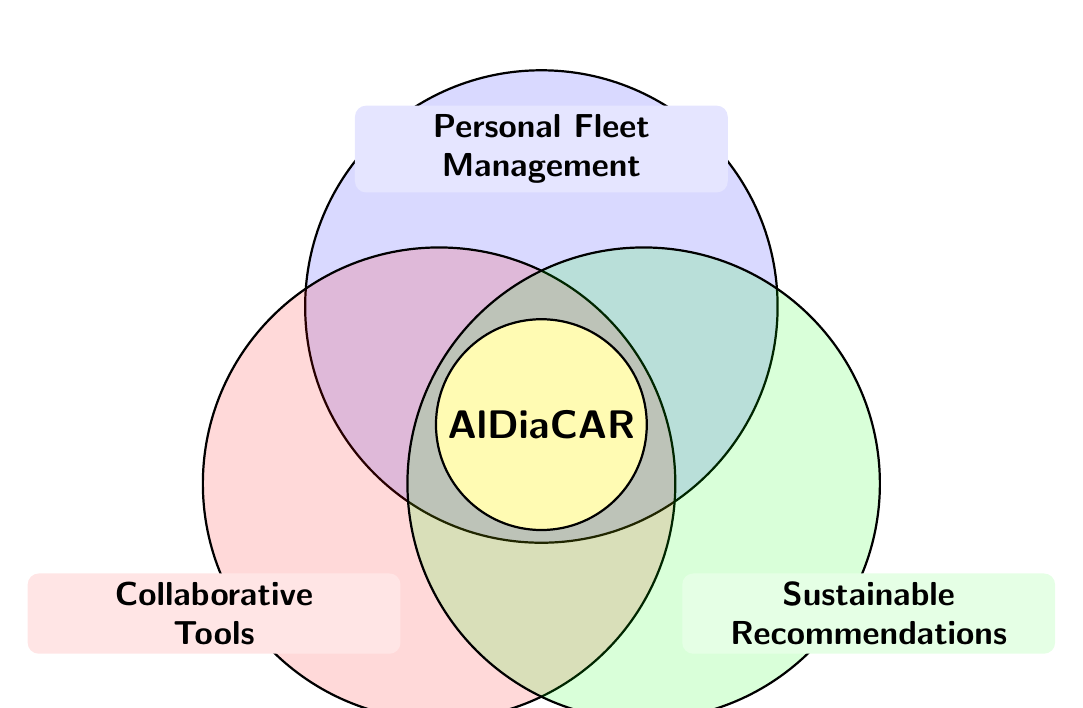
\begin{tikzpicture}[
        % Style for the main circles
        venn-circle/.style={
            draw,
            circle,
            minimum size=6cm,
            fill opacity=0.15,
            text opacity=1,
            thick
        },
        % Style for the main, overarching category labels
        category-label/.style={
            text width=4.5cm,
            align=center,
            font=\bfseries\large
        }
    ]
    
    % Draw the three main circles representing the market domains
    % Positioned at the vertices of an equilateral triangle around the origin
    \node[venn-circle, fill=blue] at (90:1.5cm) {};
    \node[venn-circle, fill=red] at (210:1.5cm) {};
    \node[venn-circle, fill=green] at (330:1.5cm) {};
    
    % Place the main category labels outside the circles, also forming an equilateral triangle
    \node[category-label, rectangle, rounded corners, fill=blue!10] at (90:3.5cm) {Personal Fleet \\ Management};
    \node[category-label, rectangle, rounded corners, fill=red!10] at (210:4.8cm) {Collaborative \\ Tools};
    \node[category-label, rectangle, rounded corners, fill=green!10] at (330:4.8cm) {Sustainable \\ Recommendations};
    
    % Highlight the central intersection, representing the market gap
    \node[font=\bfseries\Large, fill=yellow!30, circle, minimum size=2cm, draw, thick] at (0,0) {AlDiaCAR};

    \end{tikzpicture}
    \caption{Visual representation of the market gap. AlDiaCAR is positioned at the intersection of Personal Fleet Management, Sustainable Recommendations, and Collaborative Tools, a niche not currently occupied by existing solutions.}
    \label{fig:gap-analysis-diagram}
\end{figure}

To further delineate this unoccupied niche, Table \ref{tab:gap_analysis} provides a detailed comparative analysis, summarizing the limitations of existing application categories against the key requirements derived from our problem statement.

\begin{table}[h!]
    \centering
    \caption{Detailed gap analysis of existing application categories}
    \label{tab:gap_analysis}
    \resizebox{\textwidth}{!}{%
    \begin{tabular}{p{0.22\textwidth}|p{0.22\textwidth}|p{0.22\textwidth}|p{0.22\textwidth}|p{0.22\textwidth}}
        \hline
        \textbf{Application category} & \textbf{Target user} & \textbf{Core functionality} & \textbf{Sustainability focus} & \textbf{Identified gaps for AlDiaCAR Project} \\
        \hline
        Commercial Fleet Management Systems & Professional Fleet Manager (B2B) & Logistics, cost control, driver surveillance, large-scale analytics. & Primarily financial (fuel cost reduction); operational efficiency. & Prohibitively expensive and complex for personal use; lacks collaborative, non-surveillance model; misaligned UX and social context. \\
        \hline
        Personal Maintenance Apps & Individual Car Enthusiast (B2C) & Manual logging of fuel, expenses, and service for a single vehicle. & Minimal; limited to calculating fuel economy for financial tracking. & No collaborative features for shared management; poor multi-vehicle comparison; passive, utilitarian engagement model. \\
        \hline
        Eco-Routing \& Navigation Tools & General Driver / Commuter (B2C) & Calculating a fuel-efficient route for a single, generic journey. & High; focused on optimizing a single trip's route for a generic vehicle model. & Disconnected from user's actual vehicle fleet; cannot recommend the optimal vehicle, only the optimal route; lacks maintenance context. \\
        \hline
    \end{tabular}%
    }
\end{table}

\textgap

Therefore, this thesis project, \textit{AlDiaCAR}, is strategically positioned to fill this clearly defined niche. It is conceived as the first mobile application to holistically address the complex needs of an individual or family managing multiple vehicles by uniquely unifying three critical pillars of functionality into a single, user-friendly experience.

\textgap

First, it provides robust \textbf{Personal fleet management} capabilities. This goes beyond the single-vehicle logbook model by offering a centralized, collaborative dashboard where all family members can view the real-time status, location, and maintenance needs of every vehicle in the household fleet. This directly addresses the critical pain point of "shared maintenance blindness" and reduces "coordination friction."

\textgap

Second, the system incorporates \textbf{Integrated sustainability recommendations}. Unlike generic eco-routers, \textit{AlDiaCAR} leverages the detailed data of the user's specific fleet. Its recommendation engine will consider not only the destination but also the unique emissions profile, fuel efficiency, maintenance status, and regulatory constraints of each available vehicle to suggest the holistically optimal car for every journey. This transforms the application from a passive data logger into an active decision-support tool.

\textgap

Third, it implements a thoughtful \textbf{Behavioral reinforcement} layer through gamification. By embedding game-like elements such as badges, progress tracking, and positive feedback, the application aims to make sustainable choices and diligent vehicle care intrinsically rewarding. This actively encourages long-term habit formation, moving beyond mere utility to foster genuine user engagement and a collective household commitment to more sustainable mobility.

\textgap

By seamlessly combining these three pillars, the \textit{AlDiaCAR} project provides a novel and significant contribution to the field of Sustainable HCI. It offers a practical, user-centric tool designed to empower individuals and families to systematically reduce their personal transportation footprint, mitigate household friction, and manage their shared assets more efficiently and responsibly. This chapter has established the clear need and opportunity for such a solution, setting the stage for the subsequent chapters which will detail its design, implementation, and evaluation.


    % 3. Product definition
    \chapter{AlDiaCAR: System definition and phased development}

Having established the theoretical foundations and identified a distinct gap in the state-of-the-art of vehicle management applications in the preceding chapter, this chapter provides a comprehensive definition of the proposed solution: \textit{AlDiaCAR}. This chapter will serve as the architectural and functional blueprint for the project, articulating its core mission, foundational principles, and detailed feature set. The objective is to translate the conceptual framework into a tangible product specification that directly addresses the coordination frictions, maintenance blindness, and suboptimal decision-making prevalent in the modern multi-vehicle household, as exemplified by the Martínez family persona.

\textgap

The project's vision is ambitious, encompassing a wide range of functionalities from real-time coordination to intelligent, data-driven recommendations and behavioral reinforcement. To manage this complexity and ensure a methodologically sound development process, this chapter also introduces a phased implementation roadmap. This iterative approach deconstructs the complete vision into three distinct, sequential stages: the Alpha version, representing the core viable product; the Beta version, which enhances the system with intelligent features and user engagement mechanics; and finally, the Zenith release, which embodies the fully realized, feature-complete expression of the AlDiaCAR concept. This structured methodology allows for focused development, iterative testing, and the progressive validation of the project's hypotheses at each stage.

\section{The AlDiaCAR vision: A holistic framework}

The core mission of AlDiaCAR is to serve as the intelligent, collaborative "Digital garage" for the modern household. It is designed to seamlessly integrate vehicle management, user coordination, and sustainable decision-making into a single, cohesive, and effortless user experience. The system is architected upon four foundational pillars, each conceived to address a critical point of friction and inefficiency in the management of a shared, personal vehicle fleet. These pillars function interdependently to create a holistic solution that is more than the sum of its parts.

\subsection{Visual identity and design principles}

Before detailing the functional pillars, it is important to define the visual and interaction design philosophy that underpins the user experience. A consistent and thoughtful visual identity is critical for establishing user trust, ensuring usability, and creating an intuitive interface. The design of AlDiaCAR is guided by three core principles: clarity, accessibility, and encouragement. All visual elements, from the color palette to the typography, are selected to support these principles, creating a clean, modern, and non-intrusive user environment.

\textgap

Figure \ref{fig:visual-identity} presents the project's style guide, which specifies the primary and secondary color palettes, the chosen fonts for headings and body text, and the application logo. The color scheme utilizes a base of calming blues and greens to evoke a sense of reliability and sustainability, with vibrant accent colors used purposefully to draw attention to key actions and notifications.

\begin{figure}[H]
\centering
\includegraphics[width=0.9\textwidth]{images/branding/moodboard.png}
\caption{AlDiaCAR visual identity guide, defining the color palette, typography, and logo.}
\label{fig:visual-identity}
\end{figure}

\subsection{The four functional pillars}
The functionality of the AlDiaCAR system is structured around four distinct, yet interconnected, pillars. Each pillar is designed to address a specific set of pain points identified in the problem statement.

\subsubsection{Pillar 1: The shared digital key rack (Coordination)}
This foundational pillar is designed to definitively eradicate the persistent and friction-inducing "who has what car?" problem. It transforms the physical, opaque state of the household's vehicles into a transparent, digital, and universally accessible source of truth. Key functionalities include real-time vehicle status tracking, a seamless check-out/check-in protocol, and a proactive vehicle reservation system.

\subsubsection{Pillar 2: The proactive co-pilot (Intelligent recommendation)}
This pillar represents the core intelligence of the system, designed to answer the complex question, "What is the smartest vehicle choice for \textit{this specific trip}?" Its multi-vector analysis engine evaluates journeys against regulatory constraints (ZBEs), economic cost, environmental impact (CO\textsubscript{2} emissions), and maintenance awareness to provide a simple, ranked list of optimal choices.

\subsubsection{Pillar 3: The omniscient mechanic (Automated maintenance)}
This pillar acts as the household's collective, digital memory for vehicle health, ensuring that all automotive assets are consistently maintained. It combats "shared maintenance blindness" through smart maintenance profiles that track service intervals based on both time and mileage, and a shared alert system for upcoming tasks.

\subsubsection{Pillar 4: The household impact dashboard (Gamification \& analytics)}
This final pillar addresses the motivational aspects of sustainable mobility. It is designed to transform abstract data from daily use into tangible insights and positive reinforcement through a unified dashboard, personal and team-based achievements, and actionable analytics.

\section{Conceptual design and user flow wireframes}
To translate the abstract functional pillars into a concrete and user-centric interface, this section presents a series of low-fidelity wireframes. These conceptual sketches visualize the user experience of the Zenith release, illustrating the intended information architecture, component layout, and user flows for the application's most critical tasks. They serve as a visual blueprint that connects the system's defined features to its ultimate design goals.

\textgap

To translate the abstract functional pillars into a concrete and user-centric interface, this section presents a series of low-fidelity wireframes. These conceptual sketches visualize an initial, high-level vision for the user experience of the Zenith release, illustrating the potential information architecture, component layout, and user flows for the application's most critical tasks. This collection of early-stage designs, presented across Figure \ref{fig:sketches_part1} and Figure \ref{fig:sketches_part2}, serves as a visual blueprint that connects the system's defined features to its ultimate design goals.
\begin{figure}[H]
\centering
\includegraphics[width=\textwidth]{images/sketches/placeholder.png}
\label{fig:sketches_part1}
\end{figure}

\begin{figure}[H]
\centering
\includegraphics[width=\textwidth]{images/sketches/placeholder.png}
\label{fig:sketches_part2}
\end{figure}

\section{Phased implementation roadmap}

To systematically construct the comprehensive system described above, a phased development roadmap is proposed. This iterative methodology deconstructs the full feature set into three manageable and logically sequential versions. Each phase builds upon the last, allowing for focused development, targeted testing, and the potential for user feedback to inform subsequent stages. The three phases are designated as the Alpha version, the Beta version, and the Zenith release.

\subsection{The Alpha version: Establishing the core viable product}
The primary objective of the Alpha phase is to build and validate the foundational functionality of AlDiaCAR. This version is conceived as the Minimum Viable Product (MVP), focusing exclusively on solving the most acute and immediate pain points: coordination friction and shared maintenance blindness.
\textgap

\textbf{Features of the Alpha version:}
\begin{itemize}
\item \textbf{Pillar 1 (Coordination):}
\begin{itemize}
\item User and multiple vehicle registration.
\item A simple, clear dashboard showing the status of each vehicle.
\item Manual, one-tap "Check-Out" and "Check-In" functionality to update a vehicle's status between At Home and In Use. The user who checked out the vehicle is displayed.
\end{itemize}
\item \textbf{Pillar 2 (Recommendation):} This pillar is \textbf{not implemented} in the Alpha version.
\item \textbf{Pillar 3 (Maintenance):}
\begin{itemize}
\item A dedicated section for each vehicle to manually log key maintenance dates.
\item Simple, time-based push notifications when a logged date is approaching.
\end{itemize}
\item \textbf{Pillar 4 (Gamification):} This pillar is \textbf{not implemented} in the Alpha version.
\end{itemize}
The Alpha version is a digital replacement for the family's whiteboard, validating the core need for a centralized coordination hub.

\subsection{The Beta version: Enhancing intelligence and engagement}
Building upon the stable foundation of the Alpha version, the Beta phase introduces the "smart" features that define AlDiaCAR's unique value proposition.
\textgap

\textbf{Features of the Beta version (Includes all Alpha features, plus):}
\begin{itemize}
\item \textbf{Pillar 1 (Coordination):} Introduction of the vehicle \textbf{Reservation System}.
\item \textbf{Pillar 2 (Recommendation):} Implementation of an \textbf{initial Recommendation Engine} limited to \textbf{ZBE constraint analysis}.
\item \textbf{Pillar 3 (Maintenance):} Enhanced tracking with \textbf{mileage-based intervals}.
\item \textbf{Pillar 4 (Gamification):} A \textbf{first layer of gamification} with individual achievements and badges.
\end{itemize}
The Beta version transforms AlDiaCAR from a simple utility into an intelligent assistant.

\subsection{The Zenith release: The complete vision}
The Zenith release represents the culmination of the development roadmap, a feature-complete version of the application that fully realizes the initial four-pillar vision.
\textgap

\textbf{Features of the Zenith release (Includes all Beta features, plus):}
\begin{itemize}
\item \textbf{Pillar 1 (Coordination):} Polished UI/UX with potential integration into third-party calendar applications.
\item \textbf{Pillar 2 (Recommendation):} The \textbf{full, multi-factor Recommendation Engine} with cost, CO\textsubscript{2}, and maintenance awareness.
\item \textbf{Pillar 3 (Maintenance):} A shared, collaborative \textbf{Household Task List} for maintenance items.
\item \textbf{Pillar 4 (Gamification):} The complete \textbf{Household Impact Dashboard} with advanced analytics and collaborative goals.
\end{itemize}
The Zenith release is the ultimate expression of AlDiaCAR: an intelligent layer that removes friction, saves money, enhances safety, and systematically guides the family toward more sustainable mobility.


    % 4. System design
    \chapter{System design and architecture}

This chapter provides a detailed exposition of the architectural design and technical framework for the \textit{AlDiaCAR} application\footnote{A placeholder name for the application, derived from "Al Día" (up-to-date) and "Car".}. The design is fundamentally guided by the project's core objectives as defined in the preceding chapters: to deliver a cross-platform, scalable, and maintainable software solution that empowers individuals to manage and optimize their personal vehicle usage with a primary focus on enhancing sustainability and reducing operational friction.

\textgap

The following sections will deconstruct the system from a high-level perspective down to its constituent components. We will begin by outlining the overarching client-server architecture, providing a rationale for this fundamental design choice. Subsequently, we will conduct a deep dive into the specific architectural patterns employed within both the frontend and backend, justifying the decisions made to balance complexity, performance, and developer ergonomics. The chapter will also thoroughly define the data model and its current limitations, detail the communication protocols and security measures governing the data flow, and provide a comprehensive justification for the selected technology stack, including an analysis of considered alternatives. This architectural blueprint serves as the technical foundation upon which the application's features, detailed in Chapter 5, are built.

\section{High-level architecture: A client-server model}

The system is architected following a classic, robust client-server model, a paradigm in which a client requests resources and a server provides them, forming the basis of modern distributed applications \cite{Tanenbaum2011ComputerNetworks}. This approach was chosen for its clear separation of concerns, which effectively decouples the presentation layer (the user interface) from the application's core business logic and data persistence layers. This separation is paramount for achieving several key non-functional requirements. It enhances security by abstracting the database behind a controlled Application Programming Interface (API), improves scalability by allowing the client and server to be scaled independently, and provides strategic flexibility for future development, such as the creation of a web-based client or third-party integrations, without necessitating any modifications to the backend infrastructure. This decoupling is achieved through the use of well-defined APIs, which act as stable architectural boundaries that allow each component to evolve independently \cite{Martin2017CleanArchitecture}.

\textgap

The system is composed of four primary, logically distinct components:
\begin{itemize}
    \item \textbf{Frontend client:} A cross-platform mobile application, which serves as the sole point of interaction for the end-user. It is responsible for rendering the user interface, capturing user input, presenting data in a comprehensible format, and managing all communication with the backend server via a RESTful API. The use of React Native and the Expo framework enables a single codebase to target both iOS and Android platforms.
    
    \textgap

    \item \textbf{Backend server:} The central nervous system of the application. Implemented as a Node.js application using the Express.js framework, the backend serves as the authoritative hub for all operations. Its responsibilities include handling business logic, processing data, managing user authentication and authorization, and serving as the exclusive intermediary for all database interactions.
    
    \textgap

    \item \textbf{Database:} A MongoDB NoSQL database instance is utilized for all persistent data storage. This includes, but is not limited to, user profiles, detailed vehicle specifications, maintenance schedules, and trip logs. Its schema-less nature provides the flexibility required for an evolving data model.
    
    \textgap

    \item \textbf{Mock API (Development environment):} To facilitate robust, isolated, and deterministic development and testing, a secondary Node.js server is included in the development environment. This server simulates a third-party API for retrieving vehicle specifications, allowing the frontend and backend to be developed and tested without reliance on external, unpredictable, or unavailable services.
\end{itemize}

\textgap

Figure \ref{fig:high-level-arch} provides a visual representation of this architecture, illustrating the primary components and the standardized data flow protocols that connect them within the development environment.

\begin{figure}[H]
    \centering
    \begin{tikzpicture}[
        node distance=2.5cm and 3cm
    ]
    % % Components
    % \node[user] (user) {User};
    % \node[comp, right=of user] (frontend) {\textbf{Frontend Client} \\ React Native (Expo) \\ \textit{Presentation Layer}};

    % % Backend server, placed below frontend
    % \node[comp, below=of frontend, yshift=-0.5cm] (backend) {\textbf{Backend API} \\ Node.js / Express.js \\ \textit{Business Logic Layer}};

    % % Mock API server
    % \node[comp, right=of backend, xshift=1cm] (mockapi) {\textbf{Mock Car API} \\ Node.js \\ \textit{Development/Test Stub}};

    % % Database
    % \node[db, left=of backend, xshift=-1cm] (db) {MongoDB \\ \textit{Data Persistence Layer}};

    % % Docker environment container
    % \begin{pgfonlayer}{background}
    %     \node[env={Docker Environment}, fit=(backend) (db) (mockapi), inner sep=0.5cm] (dockerenv) {};
    % \end{pgfonlayer}

    % % Arrows
    % \draw[arrow] (user.east) -- (frontend.west);
    % \draw[arrow] (frontend.south) -- (backend.north) node[midway, right, xshift=0.1cm] {\textbf{REST API} \\ (HTTPS/JSON)};
    % \draw[arrow] (backend.west) -- (db.east) node[midway, below] {Mongoose ODM};
    % \draw[arrow, dashed] (frontend.east) .. controls +(east:1.5) and +(north:1) .. (mockapi.north) node[midway, above, sloped] {Mock API Call (Dev only)};

    \end{tikzpicture}
    \caption{High-level system architecture, illustrating the separation of layers and data flow.}
    \label{fig:high-level-arch}
\end{figure}

\section{Backend architecture: A Model-View-Controller approach}

The backend is architected as a monolithic RESTful API adhering to the Model-View-Controller (MVC) design pattern, a well-established architectural pattern for separating application concerns and improving modularity, as influenced by the principles of object-oriented design \cite{Gamma1995DesignPatterns}. This classical pattern was selected for its proven efficacy in organizing server-side applications, promoting a clear separation of concerns that directly maps to the project's directory structure. This organizational clarity enhances maintainability and simplifies the onboarding of future developers.

\textgap

% The request-response lifecycle within the backend follows a well-defined path, as illustrated in Figure \ref{fig:backend-lifecycle}. An incoming HTTP request from the client is first routed by Express.js to the appropriate endpoint. It then passes through a chain of middleware functions, primarily for authentication and authorization. Upon successful validation, the request is handed to the designated controller function, which contains the core business logic. The controller interacts with the Mongoose model to perform necessary database operations (Create, Read, Update, Delete - CRUD). Finally, the controller formats the response and sends it back to the client.

% \begin{figure}[H]
%     \centering
%     \includegraphics[width=\textwidth]{images/sketches/placeholder.png}
%     \caption{Sequence diagram of the backend request-response lifecycle.}
%     \label{fig:backend-lifecycle}
% \end{figure}

\subsection{Backend components}
\begin{itemize}
    \item \textbf{Routes (`/routes`):} This layer is responsible for defining the API's endpoints. It maps specific HTTP methods (GET, POST, PUT, DELETE) and URL paths to their corresponding controller functions. The design employs dedicated route files for each logical resource (e.g., \texttt{authRoutes.js}, \texttt{vehicleRoutes.js}), promoting modularity.

    \textgap
    
    \item \textbf{Controllers (`/controllers`):} Controllers form the core of the business logic. Each function within a controller is responsible for handling a specific request, orchestrating the necessary operations, and formulating the final response. In the current architecture, controllers directly interact with the Mongoose models to execute data operations and contain all business-specific logic, such as calculating maintenance alerts or processing vehicle recommendations.
    
    \textgap
    
    \item \textbf{Models (`/models`):} This layer defines the data structures (schemas) for the application's entities using Mongoose, an Object Data Modeling (ODM) library for MongoDB. The primary models are \texttt{User.js}, \texttt{Vehicle.js}, and \texttt{Trip.js}. These models are not merely schemas; they also provide a high-level abstraction for all interactions with the database, encapsulating CRUD operations.
    
    \textgap
    
    \item \textbf{Middleware (`/middleware`):} Middleware functions are executed in the intermediary stage between the router and the controller. They are primarily used for cross-cutting concerns. The most critical middleware, \texttt{authMiddleware.js}, is responsible for protecting routes by extracting and verifying the user's JSON Web Token (JWT) from the request, ensuring that only authenticated users can access protected resources.
\end{itemize}

\subsection{Architectural decision: Controller-centric business logic}
A deliberate architectural decision was made to embed all business logic directly within the controller layer, rather than abstracting it into a separate "Service Layer." For the current scope and complexity of the project, this approach offers the benefit of simplicity and reduces developmental overhead. However, it is recognized that as the application scales and business logic becomes more complex, this approach could lead to code duplication and "fat controllers." Future iterations of the system will likely require refactoring to introduce a dedicated service layer, which would encapsulate reusable business logic and be called by multiple controllers, thereby improving modularity and testability for a more complex system.

\section{Frontend architecture: A hybrid state management strategy}

The frontend client, built with React Native and Expo, employs a sophisticated and pragmatic hybrid state management strategy. This approach avoids the dogmatic application of a single pattern, instead choosing the most appropriate tool for each type of state, thereby optimizing for both developer experience and application performance.

\subsection{Global state management via React context}
For state that is truly global and required across many disparate parts of the application, the React Context API is employed. The primary use case for this is user authentication. The \texttt{AuthContext} provides the entire component tree with access to the current user's data, authentication status, and functions for logging in and out. This approach is ideal for such cross-cutting concerns because it is lightweight, built directly into the React library, and avoids the boilerplate and complexity associated with larger, third-party state management libraries like Redux, which would be excessive for the project's current needs.

\subsection{Screen-level state management (MVVM-like pattern)}
For state that is local to a specific screen or a small group of related components, the architecture follows a pattern that is conceptually aligned with Model-View-ViewModel (MVVM), where each screen manages its own state and logic, a common approach in modern client-side applications for achieving a clean separation of the view from its underlying model \cite{Garg2013ComparingPatterns}.

\textgap

For example, the "Vehicles" screen manages its own list of vehicles, its loading status, and any potential error states. It also contains the logic to fetch this data from the backend when the screen comes into focus. This encapsulation offers several advantages:
\begin{itemize}
    \item \textbf{Encapsulation and co-location:} State and the logic that manipulates it are kept together within the component that needs it, making the code easier to understand, debug, and refactor.
    \item \textbf{Performance:} It prevents the global state from becoming a bottleneck or being cluttered with data that is only relevant to a single part of the application, which in turn prevents unnecessary re-renders of unrelated components.
    \item \textbf{Testability:} Self-contained screen components are significantly easier to unit test in isolation.
\end{itemize}
This hybrid strategy provides a "best of both worlds" solution: a simple, centralized way to handle global concerns, and a scalable, encapsulated approach for managing local, feature-specific state. This approach, leveraging component-local state via Hooks and global state via the Context API, aligns with the principles of modern, declarative UI development prevalent in the React Native ecosystem \cite{Djirdeh2018FullstackReactNative}.

\section{Data architecture and modeling}

The choice of a database and the design of the data model are critical architectural decisions that directly impact the application's flexibility, scalability, and performance.

\subsection{Rationale for a NoSQL database (MongoDB)}
A NoSQL database, specifically MongoDB, was chosen over a traditional relational database (e.g., PostgreSQL) for several strategic reasons. The primary driver for this decision was the need for a flexible data schema. The domain of vehicle management involves entities with potentially diverse and evolving attributes. For example, an electric vehicle's data profile (battery capacity, charger type) is fundamentally different from that of a diesel vehicle (tank capacity, emissions standard). A NoSQL document-based model allows for these variations to exist within the same collection without requiring complex table joins or schema migrations, which is highly advantageous for a project with an iterative development roadmap. This approach aligns with the principles of aggregate-oriented databases, which prioritize scalability and development flexibility \cite{Sadalage2012NoSQLDistilled}.

\subsection{Core collections and relationships}
The data model for the current single-user scope is composed of three primary collections. The relationships are managed through ObjectIDs, which serve as foreign key equivalents.

% \begin{figure}[H]
%     \centering
%     \begin{tikzpicture}[
%         node distance=2.5cm and 3cm,
%         entity/.style={
%             rectangle, rounded corners, draw=black, very thick,
%             minimum width=4cm, minimum height=2cm, align=left,
%             text width=5cm, fill=blue!10, drop shadow
%         },
%         arrow/.style={-{Latex[length=3mm]}, very thick}
%     ]

%     % Entities
%     \node[entity] (user) {\textbf{User Collection} \\ \texttt{\_id: ObjectId (PK)} \\ \texttt{name: String} \\ \texttt{email: String (unique)} \\ \texttt{password: String (hashed)} \\ \texttt{achievements: [String]}};
%     \node[entity, right=of user, xshift=2cm] (vehicle) {\textbf{Vehicle Collection} \\ \texttt{\_id: ObjectId (PK)} \\ \texttt{owner: ObjectId (FK -> User)} \\ \texttt{make: String} \\ \texttt{model: String} \\ \texttt{year: Number} \\ \texttt{fuelType: String (Enum)} \\ \texttt{emissions: Number (gCO2/km)} \\ \texttt{maintenance: \{...\} (Embedded)} };
%     \node[entity, below=of vehicle] (trip) {\textbf{Trip Collection} \\ \texttt{\_id: ObjectId (PK)} \\ \texttt{driver: ObjectId (FK -> User)} \\ \texttt{vehicle: ObjectId (FK -> Vehicle)} \\ \texttt{distance: Number} \\ \texttt{date: Date}};

%     % Relationships
%     \draw[arrow] (user.east) -- (vehicle.west) node[midway, above, text width=2cm, align=center] {1..n \\ owns};
%     \draw[arrow] (vehicle.south) -- (trip.north) node[midway, right] {1..n \\ used in};
%     \path (user.south) edge[arrow, bend right=30] node[midway, left] {1..n \\ logs} (trip.west);

%     \end{tikzpicture}
%     \caption{Detailed Data Model illustrating collections, key fields, and relationships.}
%     \label{fig:data-model-detailed}
% \end{figure}

\subsection{Modeling maintenance: The embedded document approach}
In the current design, maintenance information is modeled as a single, embedded sub-document within each \texttt{Vehicle} document. Each key within this sub-document represents a specific maintenance task (e.g., `oilChange`, `itvInspection`), and its value stores the corresponding due date or mileage. This denormalized approach was chosen for its simplicity and performance. It allows all maintenance data for a vehicle to be retrieved in a single database query, avoiding the need for complex joins or additional lookups that would be required with a separate `MaintenanceItem` collection. While this approach is highly efficient for the current feature set, it may be revisited if future requirements necessitate more complex querying or history tracking of maintenance tasks.

\subsection{Architectural limitation and future work: The household model}
A significant and acknowledged limitation of the current data architecture is its exclusive focus on a single-user context. Users are standalone entities, and there is no data structure to group them into a "household" or to model the shared ownership or use of vehicles. This design decision was made to constrain the initial project scope to a manageable size.

\textgap

Evolving the system to a full multi-user, collaborative "household" model represents the most significant future architectural challenge. This would necessitate substantial changes to the data model, including:
\begin{enumerate}
    \item The introduction of a new \textbf{\texttt{Household}} collection.
    \item A mechanism to link multiple \texttt{User} documents to a single \texttt{Household}.
    \item A robust invitation and membership management system.
    \item A re-evaluation of the `owner` field on the \texttt{Vehicle} collection to support shared ownership or distinguish between an owner and authorized drivers.
    \item A more granular authorization model (potentially Role-Based Access Control) to manage permissions within a household.
\end{enumerate}
This future work is a logical extension of the current system and is a primary consideration for post-thesis development.

\section{API design and security protocols}

The design of the Application Programming Interface (API) and its underlying security protocols are critical for ensuring reliable communication and protecting user data.

\subsection{API design: RESTful principles}
The API is designed following REST (Representational State Transfer) principles, adhering to the constraints of statelessness, resource-based addressing, and a uniform interface as defined in the foundational architectural style \cite{Fielding2000REST}. It uses standard HTTP methods (GET, POST, PUT, DELETE) for operations, leverages URL paths to identify resources (e.g., \texttt{/api/vehicles}), and uses standard HTTP status codes to communicate the outcome of requests. All data is exchanged in the JSON format. This adherence to web standards makes the API predictable, easy to consume by clients, and broadly understood.

\subsection{Authentication: JWT in HTTP-only cookies}
User authentication is managed via JSON Web Tokens (JWTs). Upon successful login, the backend server generates a signed JWT containing the user's ID and sends it back to the client in a secure, \textbf{HTTP-Only} cookie. This cookie is automatically included by the browser/client in all subsequent requests to the server. The HTTP-Only flag is a crucial security measure, as it prevents the token from being accessed by client-side JavaScript, thereby mitigating the risk of Cross-Site Scripting (XSS) attacks.

\subsection{Authorization: Ownership-based access control (OBAC)}
The system's authorization strategy is Ownership-Based Access Control. Once a user is authenticated (their identity is confirmed via JWT), the authorization middleware performs a second check for any request that attempts to access or modify a specific resource (like a vehicle). The middleware ensures that the authenticated user's ID matches the \texttt{owner} field of the requested resource. If they do not match, the request is rejected with a `403 Forbidden` status. This simple yet effective model ensures that users can only interact with their own data.

\subsection{Standardized error handling}
A consistent error handling strategy is employed to ensure that the client can reliably interpret and respond to issues. The API uses standard HTTP status codes in conjunction with a structured JSON error body.

\begin{table}[h!]
    \centering
    \caption{Standard API HTTP status codes and meanings}
    \begin{tabular}{l|p{0.7\textwidth}}
        \hline
        \textbf{Status Code} & \textbf{Meaning in AlDiaCAR Context} \\
        \hline
        200 OK & The request was successful (e.g., successful GET request). \\
        \hline
        201 Created & The request was successful and a new resource was created (e.g., successful POST to create a vehicle). \\
        \hline
        400 Bad Request & The request could not be understood by the server due to malformed syntax (e.g., missing required fields in the request body). \\
        \hline
        401 Unauthorized & The request requires user authentication. The client has not provided a valid JWT. \\
        \hline
        403 Forbidden & The user is authenticated, but does not have permission to access the requested resource (OBAC failure). \\
        \hline
        404 Not Found & The requested resource could not be found on the server. \\
        \hline
        500 Internal Server Error & A generic error message, given when an unexpected condition was encountered on the server. \\
        \hline
    \end{tabular}
\end{table}

\section{Technology stack justification}

The selection of each technology in the stack was the result of a deliberate evaluation of the project's specific requirements against the strengths and weaknesses of available options.

\begin{itemize}
    \item \textbf{React Native (with Expo):} Chosen for its primary benefit of cross-platform development, allowing a single JavaScript/TypeScript codebase to generate native applications for both iOS and Android. This drastically reduces development time and effort. Expo was specifically included to abstract away the complexities of native build configurations, further accelerating the development cycle.
    \newline\textit{Considered Alternative: Flutter.} Flutter was a strong contender but was ultimately not selected due to the project's reliance on the vast JavaScript/React ecosystem and the desire for language synergy between the frontend and backend.
    
    \textgap
    
    \item \textbf{Node.js with Express.js:} Selected for the backend due to its non-blocking, event-driven architecture, which provides excellent performance for I/O-heavy operations typical of an API server. The use of JavaScript/TypeScript creates a seamless, full-stack development experience, allowing for shared code and libraries.
    \newline\textit{Considered Alternative: Python with Django/Flask.} While powerful, this stack was passed over to maintain language consistency across the entire project, which simplifies the development toolchain.
    
    \textgap
    
    \item \textbf{MongoDB:} As previously detailed, MongoDB was chosen for its flexible document-based schema, which is highly suited to the evolving and varied data structures of vehicle profiles. Its inherent scalability is also a significant advantage for future growth.
    \newline\textit{Considered Alternative: PostgreSQL.} A relational database like PostgreSQL was considered for its data integrity features (ACID compliance). However, the anticipated need for schema flexibility was deemed a more critical requirement for this project, making MongoDB the superior choice.
    
    \textgap

    \item \textbf{Docker:} Docker and Docker Compose are utilized to containerize the backend services. This practice is a key enabler of modern Continuous Delivery pipelines, as it eliminates environmental discrepancies and simplifies the deployment process \cite{Humble2010ContinuousDelivery}. This ensures a consistent, reproducible, and isolated development environment, eliminating "it works on my machine" problems and simplifying the setup process for any developer working on the project.
\end{itemize}

\section{Architectural considerations for external integrations}

While the current version of the application operates as a self-contained system, the Zenith Release vision requires integration with several third-party services. The architecture is designed with this future extensibility in mind. The primary external integrations required are:

\begin{itemize}
    \item \textbf{Mapping and Routing Services:} To calculate trip distances and potentially offer turn-by-turn navigation.
    \item \textbf{Low Emission Zone (ZBE) Data Services:} To fetch real-time, geo-located data on ZBE boundaries and access rules.
    \item \textbf{Fuel Price Data Services:} To provide real-time local fuel prices for accurate cost calculations.
\end{itemize}

\textgap

To manage these future integrations without creating tight coupling, the backend architecture will employ the \textbf{Adapter Pattern}. For each type of external service, a dedicated "adapter" or "connector" module will be created. This module will serve as an intermediary, translating the application's internal requests into the specific format required by the external API and translating the external API's response back into a standardized format for the application. This abstraction ensures that if a provider (e.g., for fuel price data) needs to be changed in the future, only the corresponding adapter module needs to be rewritten; the core business logic of the application remains untouched. This design promotes modularity, testability, and long-term maintainability.


    % 5. Code implementation
    \chapter{Implementation details}

This chapter transitions from the abstract design of Chapter 3 to the concrete technical implementation of the \textit{AlDiaCAR} system. It provides a detailed walkthrough of the project's source code, explaining the structure, key modules, and programming patterns used in both the backend and frontend.

\section{Project structure overview}

The project is organized as a monorepo, a single repository containing all the code for the system. This approach simplifies dependency management and streamlines development across the different parts of the application. The high-level directory structure is shown in Figure \ref{fig:dirtree}.

\begin{figure}[h!]
\dirtree{%
.1 .
.2 config/ \textit{(Docker service configurations)}.
.3 mongo-express-config.js.
.2 docker/ \textit{(Local environment definition)}.
.3 docker-compose.yaml.
.2 src/ \textit{(Main source code)}.
.3 backend/ \textit{(Node.js REST API)}.
.4 controllers/.
.4 middleware/.
.4 models/.
.4 routes/.
.4 server.js.
.3 frontend/ \textit{(React Native mobile app)}.
.4 app/ \textit{(Expo file-based routes)}.
.4 components/.
.4 context/.
.4 localization/.
.2 tests/ \textit{(Automated tests)}.
.3 backend/ \textit{(Jest tests)}.
.3 frontend/ \textit{(Playwright E2E tests)}.
.2 package.json \textit{(Root monorepo scripts)}.
}
\caption{High-level project directory structure.}
\label{fig:dirtree}
\end{figure}

The \texttt{src} directory cleanly separates the \texttt{backend} and \texttt{frontend} concerns. The \texttt{docker} directory ensures a reproducible development environment, while the \texttt{tests} directory houses the quality assurance framework.

\section{Backend implementation (Node.js)}

The backend is a RESTful API built with Node.js and the Express.js framework. It is responsible for all business logic, data persistence, and security.

\subsection{Data models (Mongoose)}
Data schemas are defined in \texttt{src/backend/models/} using Mongoose. The principal models are \texttt{User.js}, \texttt{Vehicle.js}, and \texttt{Trip.js}. A key feature is the use of Mongoose's \texttt{timestamps} option in the User schema to automatically manage \texttt{createdAt} and \texttt{updatedAt} fields. The password field uses \texttt{select: false} to prevent it from ever being sent in an API response. The full schema definitions are detailed in Appendix B.

\subsection{Controllers and business logic}
Controllers, located in \texttt{src/backend/controllers/}, contain the core logic for each API endpoint. While many controllers perform standard CRUD operations, some, like \texttt{tripController.js}, encapsulate more complex business logic. The \texttt{logSimulatedTrip} function demonstrates how a single API call can trigger multiple state changes across the system.

\begin{lstlisting}[language=JavaScript, caption={Core logic from \texttt{tripController.js}}]
// 1. UPDATE VEHICLE MAINTENANCE METRICS
if (vehicle.upcomingMaintenance) {
  if (vehicle.upcomingMaintenance.brakes?.distance) {
    vehicle.upcomingMaintenance.brakes.distance -= distance;
  }
  // ... other distance-based counters are reduced
}

// 2. CREATE THE TRIP RECORD
const calculatedEmissions = distance * (vehicle.emissions || 150);
await Trip.create({ driver: userId, vehicle: vehicleId, distance, ... });

// 3. UPDATE USER STATS & GRANT ACHIEVEMENTS
user.stats.distanceTraveled += distance;
const achievementsToGrant = [];
if (!user.achievements.includes('FIRST_TRIP')) {
  achievementsToGrant.push('FIRST_TRIP');
}
if (oldDistance < 1000 && user.stats.distanceTraveled >= 1000) {
  achievementsToGrant.push('DIST_1000');
}
if (achievementsToGrant.length > 0) {
  user.achievements.push(...achievementsToGrant);
}

// 4. SAVE ALL CHANGES ATOMICALLY
await Promise.all([vehicle.save(), user.save()]);
\end{lstlisting}

This function shows how logging a trip correctly decrements maintenance counters on the vehicle, creates a new trip record, and updates the user's statistics and achievements, all within a single transaction. Figure \ref{fig:data-flow-trip} illustrates this interaction.

\begin{figure}[h!]
    \centering
    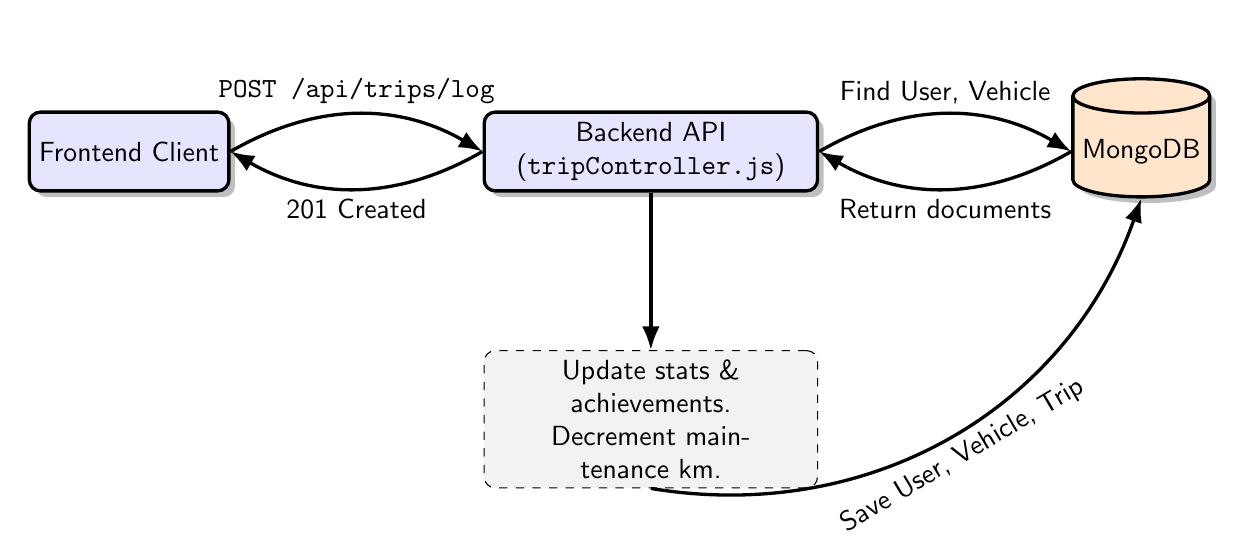
\begin{tikzpicture}[
        node distance=2cm and 3.2cm, 
        font=\sffamily,
        proc/.style={
            rectangle, rounded corners, draw, dashed, fill=gray!10,
            text width=4cm, align=center, minimum height=1.5cm
        }
    ]
        \node (client) [comp, minimum width=2.5cm, text width=2.3cm] {Frontend Client};
        \node (backend) [comp, right=of client, text width=4cm] {Backend API \\ (\texttt{tripController.js})};
        \node (db) [db, right=of backend] {MongoDB};

        \draw[arrow, bend left=30] (client.east) to node[midway, above, sloped] {\texttt{POST /api/trips/log}} (backend.west);
        \draw[arrow, bend left=30] (backend.west) to node[midway, below, sloped] {201 Created} (client.east);
        
        \draw[arrow, bend left=30] (backend.east) to node[midway, above, sloped] {Find User, Vehicle} (db.west);
        \draw[arrow, bend left=30] (db.west) to node[midway, below, sloped] {Return documents} (backend.east);
        
        \node[proc, below=of backend, node distance=2cm] (logic) {Update stats \& achievements. \\ Decrement maintenance km.};
        \draw[arrow] (backend) -- (logic);
        
        \draw[arrow, bend right=40] (logic.south) to node[midway, below, sloped] {Save User, Vehicle, Trip} (db.south);

    \end{tikzpicture}
    \caption{Sequence diagram for the trip logging data flow.}
    \label{fig:data-flow-trip}
\end{figure}

\subsection{API routes and middleware}
Routes defined in \texttt{src/backend/routes/} map the API endpoints to controller functions. The most critical middleware, \texttt{authMiddleware.js}, protects these routes. It extracts the JWT from an \texttt{HttpOnly} cookie, verifies it, and attaches the user's ID to the request object. This makes the user's identity available to any protected controller.

\section{Frontend implementation (React Native)}

The frontend is a cross-platform mobile application developed using React Native with the Expo framework and TypeScript for static typing.

\subsection{Navigation and screen structure}
The application uses Expo's file-based router. Directories and files within \texttt{src/frontend/app/} automatically become routes.
\begin{itemize}
    \item \textbf{Layouts (`\_layout.tsx`):} These files define the shell UI, such as the main tab bar defined in \texttt{app/(tabs)/\_layout.tsx}.
    \item \textbf{Authentication flow (`app/(auth)`):} A route group for the login and register screens, active when a user is not authenticated.
    \item \textbf{Main screens (`app/(tabs)`):} Represent the core features. A key pattern used is \texttt{useFocusEffect} from Expo Router to re-fetch data whenever a screen comes into view, ensuring data is always fresh after an update (e.g., after adding a new vehicle).
\end{itemize}

\subsection{State management and API communication}
Global state for user authentication is managed via React's Context API in \texttt{context/AuthContext.tsx}. This provider stores the user's authentication status and profile information. Communication with the backend is handled using the \texttt{axios} library, which is configured with \texttt{withCredentials: true} to automatically handle the sending and receiving of authentication cookies.

\section{Integration and deployment}

\subsection{Local development with Docker}
To ensure a consistent development environment, the project utilizes Docker and Docker Compose. The \texttt{docker/docker-compose.yaml} file defines all services required to run the application stack locally, including the backend, frontend, database, and the Mongo Express GUI. A developer can start the entire stack with a single command: \texttt{docker-compose up}.

\subsection{Deployment strategy}
While the current focus is a robust prototype, a potential production deployment strategy would involve:
\begin{itemize}
    \item \textbf{Backend:} Containerizing the Node.js application and deploying it to a Platform-as-a-Service (PaaS) like Heroku or a container orchestrator.
    \item \textbf{Database:} Using a managed database service like MongoDB Atlas.
    \item \textbf{Frontend:} Building the mobile application for production using Expo Application Services (EAS) and submitting the binaries to the app stores.
\end{itemize}

\section{Testing strategy and implementation}
The \texttt{tests/} directory houses a multi-layered testing strategy. For full details on the specific test cases, see Appendix D.
\begin{itemize}
    \item \textbf{Backend unit \& Integration tests:} The \texttt{tests/backend/} directory uses Jest to test modules in isolation and Supertest to test API endpoint integration.
    \item \textbf{Frontend E2E tests:} The \texttt{tests/frontend/} directory is configured for Playwright, which runs automated tests that simulate key user journeys in a real browser environment.
\end{itemize}

\section{Security and privacy considerations}
Security is implemented through several mechanisms:
\begin{itemize}
    \item \textbf{Password hashing:} The \texttt{bcryptjs} library is used to securely hash and salt user passwords.
    \item \textbf{Authentication:} JWTs are stored in secure, \texttt{HttpOnly} cookies, which helps mitigate cross-site scripting (XSS) attacks.
    \item \textbf{Route protection:} The \texttt{authMiddleware} ensures that only authenticated users can access protected endpoints.
    \item \textbf{Environment variables:} Sensitive information like database connection strings and JWT secrets are managed via \texttt{.env} files and are not committed to version control.
\end{itemize}



\section{Development effort and cost analysis}

While this project was undertaken within an academic context, it is valuable to perform a cost analysis to estimate the resources required to develop a market-ready product based on the AlDiaCAR concept. This section provides a high-level budget estimation, breaking down the costs associated with the development of the "Thesis-Grade Beta" (the scope implemented for this project) and projecting the additional investment needed to achieve the full Zenith release.

\subsection{Methodology and assumptions}

The budget is calculated based on a team of freelance professionals based in Spain, with standard market rates for software development roles. The estimation is based on the hours required for each key phase of the project: design, development, and project management.

The following roles and hourly rates are assumed:
\begin{itemize}
\item \textbf{Project manager / Product owner:} Responsible for requirements, planning, and oversight. Rate: €50/hour.
\item \textbf{UI/UX Designer:} Responsible for visual identity, wireframing, and creating high-fidelity mockups. Rate: €35/hour.
\item \textbf{Backend developer:} Responsible for the server, API, and database architecture. Rate: €40/hour.
\item \textbf{Frontend (Mobile) developer:} Responsible for the React Native application. Rate: €40/hour.
\end{itemize}

\subsection{Estimated development costs}

Table \ref{tab:development_costs} outlines the estimated hours and costs for the development of the Thesis-Grade Beta (representing the completed Alpha and Beta phases) and the projected additional effort required to complete the Zenith release.

\begin{table}[H]
\small
\centering
\caption{Estimated development costs by phase}
\label{tab:development_costs}
\begin{tabular}{>{\raggedright\arraybackslash}p{3cm} | >{\centering\arraybackslash}p{1.5cm} >{\centering\arraybackslash}p{1.5cm} | >{\centering\arraybackslash}p{1.5cm} |  >{\centering\arraybackslash}p{1.5cm} >{\centering\arraybackslash}p{1.5cm}}
\hline
\textbf{Role} & \textbf{Hours (Beta)} & \textbf{Hours (Zenith add-on)} & \textbf{Rate (€/hr)} & \textbf{Subtotal (Beta)} & \textbf{Subtotal (Zenith add-on)} \\[2pt]
\hline
Project manager & 40 hrs & 60 hrs & €50 & €2,000 & €3,000 \\[0.9cm]
UI/UX Designer & 30 hrs & 40 hrs & €35 & €1,050 & €1,400 \\[0.9cm]
Backend developer & 120 hrs & 100 hrs & €40 & €4,800 & €4,000 \\[0.9cm]
Frontend developer & 120 hrs & 100 hrs & €40 & €4,800 & €4,000 \\[0.9cm]
\hline
\textbf{Total person-hours} & \textbf{310 hrs} & \textbf{300 hrs} & --- & --- & --- \\[2pt]
\textbf{Subtotal labor costs} & --- & --- & --- & \textbf{€12,650} & \textbf{€12,400} \\[2pt]
\hline
\multicolumn{5}{r}{\textbf{Projected total for Zenith release:}} & \textbf{€25,050} \\
\hline
\end{tabular}
\end{table}

The development of the Thesis-Grade Beta, which includes the critical household data model, the reservation system, and the full multi-factor recommendation engine, is estimated to require approximately 310 person-hours, resulting in a cost of €12,650.

\textgap

To complete the Zenith release, which would involve integrating live third-party APIs, building the full graphical analytics dashboard, and implementing the collaborative gamification layer, an additional 300 person-hours are projected. This would represent a further investment of €12,400, bringing the total estimated development cost for a market-ready Zenith version to €25,050.

\subsection{Other associated costs}

Beyond direct development labor, a production-grade application would incur other initial and ongoing costs. These are summarized in Table \ref{tab:other_costs}.

\begin{table}[H]
\normalsize
\centering
\caption{Other costs annual estimation}
\label{tab:other_costs}
\begin{tabular}{l|p{6.6cm}|r}
\hline
\textbf{Category} & \textbf{Description} & \textbf{Est. cost (p.a.)} \\
\hline
Infrastructure & Server hosting (PaaS), managed database (MongoDB atlas) & €600 \\
Third-Party APIs & Google Maps API, ZBE data provider, fuel price API & €500 - €1,500 \\
App store fees & Apple developer program, Google Play developer account & €125 \\
Contingency (15\%) & For unforeseen development challenges and scope changes & €3,757 (initial) \\
\hline
\textbf{Total (First year)} & & \textbf{€4,982 - €5,982} \\
\hline
\end{tabular}
\end{table}

\textgap


    % 6. Validation
    \chapter{Results and validation}

This chapter presents the results of the implementation phase, validating the functionality of the \textit{AlDiaCAR} prototype against the objectives defined in the preceding chapters. The validation process serves two primary purposes: first, to confirm that the system's key features are operational and have been implemented correctly according to the architectural design; and second, to demonstrate that these features effectively address the core problem statement. This chapter provides visual evidence of the working frontend through a walkthrough of the core user journeys, complemented by a summary of the automated tests that verify the backend logic and the integrity of the system as a whole.

\section{Frontend validation via core user workflows}

The most direct method for validating the application's success is to demonstrate its functionality from the end-user's perspective. The following sections use screenshots from the running application to provide tangible evidence that the primary features have been successfully implemented and that the core user workflows are operational.

\subsection{User onboarding and household management}
The user journey begins with registration. As per the system's architecture, upon creating an account, each user is automatically assigned to a new, personal household. This establishes the foundational collaborative entity from the outset. The user can then manage their household, invite others, or join an existing household. This workflow directly validates the implementation of the `Household` data model, which is central to the project's collaborative goals.

\textgap

Figure \ref{fig:login-screen} shows the application's login screen, the entry point for authenticated users. Upon successful login, the user can navigate to their profile, as shown in Figure \ref{fig:profile-household-screen}. This screen serves as the central hub for identity and household management, displaying the user's details, the current household's name, its unique join code for inviting others, and a list of current members. This screen confirms that the authentication, data retrieval, and household association processes are functioning correctly.

\begin{figure}[H]
    \centering
    \includegraphics[width=0.4\textwidth]{images/results/login_screen.png}
    \caption{The user login screen, serving as the gateway to the application.}
    \label{fig:login-screen}
\end{figure}

\begin{figure}[H]
    \centering
    \includegraphics[width=0.45\textwidth]{images/results/profile_household_screen.png}
    \caption{The user profile screen, displaying personal details and the household management card with its unique join code and member list.}
    \label{fig:profile-household-screen}
\end{figure}

\subsection{Vehicle fleet management}
A core requirement of the system is to provide users with a centralized tool to manage their personal fleet of vehicles. The "Vehicles" tab provides this functionality, validating the system's CRUD (Create, Read, Update, Delete) capabilities for vehicles. Users can view all vehicles associated with their household, add new vehicles, and edit or delete existing ones.

\textgap

Figure \ref{fig:vehicle-list-screen} shows the main vehicle list, providing a complete, at-a-glance overview of the household's automotive assets. From this screen, the user can initiate the process of adding a new car, which leads to the form shown in Figure \ref{fig:add-vehicle-screen}. This workflow demonstrates a key feature: the system first requires basic vehicle information and then simulates a call to an external service (via the Mock API) to fetch technical specifications like the emission factor, which is crucial for the recommendation engine.

\begin{figure}[H]
    \centering
    \includegraphics[width=0.45\textwidth]{images/results/vehicle_list_screen.png}
    \caption{The main vehicle management screen, displaying a list of all vehicles registered to the household.}
    \label{fig:vehicle-list-screen}
\end{figure}

\begin{figure}[H]
    \centering
    \includegraphics[width=0.45\textwidth]{images/results/add_vehicle_screen.png}
    \caption{The two-step process for adding a new vehicle, including fetching technical specifications from the mock external API.}
    \label{fig:add-vehicle-screen}
\end{figure}

\subsection{Coordination and vehicle status dashboard}
To directly address the problem of coordination friction, the "Home" tab serves as a real-time vehicle status dashboard. This interface, shown in Figure \ref{fig:status-dashboard-screen}, provides all household members with immediate and transparent visibility into the current state of each vehicle: `At Home`, `In Use`, or `Reserved`.

\textgap

This screen validates the implementation of Pillar 1. Users can perform one-tap "Check-Out" and "Check-In" actions to update a vehicle's status. Furthermore, the dashboard provides the interface for the vehicle reservation system. As shown in Figure \ref{fig:reservation-modal}, a user can select an available vehicle and reserve it for a future time slot, which immediately updates its status for all other household members, preventing scheduling conflicts and enabling proactive planning.

\begin{figure}[H]
    \centering
    \includegraphics[width=0.6\textwidth]{images/results/status_dashboard_screen.png}
    \caption{The main status dashboard, providing real-time visibility into the availability of each household vehicle.}
    \label{fig:status-dashboard-screen}
\end{figure}

\begin{figure}[H]
    \centering
    \includegraphics[width=0.45\textwidth]{images/results/reservation_modal.png}
    \caption{The reservation modal, allowing a user to book an available vehicle for a specific future time slot.}
    \label{fig:reservation-modal}
\end{figure}

\subsection{Proof-of-concept for recommendation}
The validation of the system's core hypothesis—that an intelligent engine can guide sustainable choices—is demonstrated through the "Routes" workflow. As established in the project's scope, this implementation serves as a vertical slice proof-of-concept for the Pillar 2 recommendation engine.

\textgap

The user first selects a trip from a set of predefined locations, one of which is inside a hardcoded ZBE, as shown in Figure \ref{fig:route-planning-screen}. The application then sends this information to the backend, which processes it against the ZBE rules. The result, displayed in Figure \ref{fig:recommendation-results-screen}, is a ranked list of available vehicles. In this example, the destination is inside the ZBE, so the system has automatically filtered out non-compliant vehicles and presents only the eligible, hybrid car as the "Best Choice," thus validating the core constraint-based filtering logic.

\begin{figure}[H]
    \centering
    \includegraphics[width=0.45\textwidth]{images/results/route_planning_screen.png}
    \caption{The route planning interface, where the user selects a trip from a list of predefined demonstration locations.}
    \label{fig:route-planning-screen}
\end{figure}

\begin{figure}[H]
    \centering
    \includegraphics[width=0.45\textwidth]{images/results/recommendation_results_screen.png}
    \caption{The recommendation results screen. A "ZBE DETECTED" warning is displayed, and the list of vehicles is filtered accordingly.}
    \label{fig:recommendation-results-screen}
\end{figure}

\subsection{Statistics and gamification}
Finally, the "Stats" tab validates the foundational elements of Pillar 4. This screen, shown in Figure \ref{fig:stats-screen}, aggregates data from the user's logged trips to provide key performance indicators, such as total distance traveled and total CO\textsubscript{2} emissions. It also displays the user's earned achievements, confirming that the backend logic for tracking user actions and granting awards is functioning correctly. This serves as the data collection and feedback mechanism upon which the full analytics dashboard and collaborative gamification of the Zenith release would be built.

\begin{figure}[H]
    \centering
    \includegraphics[width=0.45\textwidth]{images/results/stats_screen.png}
    \caption{The statistics and achievements screen, providing the user with tangible feedback on their activity and progress.}
    \label{fig:stats-screen}
\end{figure}

\section{Backend and End-to-End validation}
To validate the system's logic and the integrity of the integration between the frontend and backend, a suite of automated tests was executed.

\subsection{Backend integration testing}
The backend test suite was run using Jest and Supertest to verify the correctness of the API endpoints in a controlled environment. The tests cover critical business logic, including authentication, household management, and the core recommendation algorithm. Figure \ref{fig:jest-results} shows the output from the test runner, confirming that all implemented tests passed successfully. This result validates that the server-side logic is robust and performs as expected according to the system design.

\begin{figure}[H]
    \centering
    \includegraphics[width=0.9\textwidth]{images/results/jest_test_results.png}
    \caption{Output from the Jest test runner, confirming the successful execution of the backend integration test suite.}
    \label{fig:jest-results}
\end{figure}

\subsection{End-to-End (E2E) testing}
To validate the complete user journey from the user interface to the database and back, E2E tests were conducted using the Playwright framework. These tests automate a web browser to perform critical user flows such as registration, login, and adding a vehicle. Figure \ref{fig:playwright-results} displays the summary report from the Playwright test execution, indicating that all critical-path user journeys completed without errors. This validates the seamless integration between the frontend and backend components.

\begin{figure}[H]
    \centering
    \includegraphics[width=0.9\textwidth]{images/results/playwright_test_results.png}
    \caption{Summary report from the Playwright E2E test suite, showing that all critical user flows passed successfully.}
    \label{fig:playwright-results}
\end{figure}

\section{Validation summary}
The combination of visual confirmation from the frontend walkthroughs and the successful execution of the automated test suites confirms that the AlDiaCAR prototype successfully implements its core objectives. The system effectively provides a collaborative framework for household vehicle management and validates the technical feasibility of its innovative recommendation engine. Table \ref{tab:validation-summary} maps the core project objectives to their implemented and validated status.

\begin{table}[H]
    \centering
    \caption{Summary of validated project objectives}
    \label{tab:validation-summary}
    \resizebox{\textwidth}{!}{
    \begin{tabular}{p{0.35\textwidth}|p{0.5\textwidth}|p{0.15\textwidth}}
        \hline
        \textbf{Objective} & \textbf{Validation Method} & \textbf{Status} \\
        \hline
        Mitigate coordination friction & Frontend screenshots (Status dashboard, reservation modal), E2E tests (Playwright) & Implemented \\
        \hline
        Combat maintenance blindness & Frontend screenshots (Maintenance modal), Backend tests (Jest) & Implemented \\
        \hline
        Address inefficient selection & Frontend screenshots (Recommendation screen), Backend tests (Jest) & Implemented \\
        \hline
        Establish collaborative framework & Frontend screenshots (Household card), Backend tests (Jest), E2E tests & Implemented \\
        \hline
        Gamification foundation & Frontend screenshot (Stats screen), Backend tests (Jest) & Implemented \\
        \hline
    \end{tabular}
    }
\end{table}


    % 7. Management and planning
    \chapter{Project management and planning}

This chapter details the project management framework, planning methodology, and execution strategy employed throughout the development of the \textit{AlDiaCAR} thesis project. It outlines the processes used for task identification, scheduling, and resource management, and provides a transparent account of the strategic decisions made to navigate the challenges inherent in a research-oriented software development endeavor.

\section{Methodology}

The project was executed following an exploratory and iterative methodology. This approach was deliberately chosen over a more traditional, rigid waterfall model. A waterfall methodology, with its sequential and inflexible phases, was deemed fundamentally unsuitable for this project, where the process of writing the thesis and developing the software artifact were deeply intertwined. Requirements and architectural insights often emerged during the implementation process itself, necessitating a flexible approach that allowed for continuous refinement.

\textgap

This iterative methodology provided the necessary adaptability. By developing the system in progressive cycles, it was possible to build and validate components incrementally, with the writing of the thesis and the coding of the application informing each other. This progressive development and validation strategy was crucial for ensuring that the final research artifact was both robust and directly aligned with the project's central academic hypotheses, even as the understanding of the problem space deepened over time.

\section{Project phases and task organization}

To structure the project and ensure comprehensive coverage of all necessary activities, the work was logically deconstructed into five primary phases. This approach, analogous to a Work Breakdown Structure (WBS) \footnote{\href{https://www.projectmanager.com/guides/work-breakdown-structure}{A Guide to Work Breakdown Structure (WBS)}}, provided a clear sequence for the project's execution, grouping activities from initial research to final documentation.

\begin{itemize}
\item \textbf{Phase 1: Research and state-of-the-art analysis.} This initial and foundational phase involved a comprehensive review of academic literature and existing market solutions. It included a detailed analysis of competing applications, research into the theoretical foundations of persuasive technology and Green IT, and the formal identification of the market gap that this thesis aims to address. The outputs of this work are detailed in Chapter 2.
\textgap
\item \textbf{Phase 2: System design and architecture.} This phase encompassed all high-level planning and design activities. Responsibilities included the definition of the client-server architecture, the selection of the technology stack, the formal modeling of the application's data structures, and the conceptual design of the user interface and user experience (UI/UX)\footnote{\href{https://flatironschool.com/blog/what-is-ux-ui-design/}{What is UX / UI Design? }} through the creation of wireframes and a visual style guide. This work corresponds to the material presented in Chapters 3 and 4.
\textgap
\item \textbf{Phase 3: Proof-of-concept implementation.} This phase represented the core software development effort. The primary goal was the implementation of a focused prototype to validate the most novel and complex aspects of the system. This included building the backend API, the frontend mobile application, and the necessary database schemas. The technical details of this implementation are documented in Chapter 5.
\textgap
\item \textbf{Phase 4: Testing and validation.} This phase focused on ensuring the quality, correctness, and robustness of the software artifact. It included the implementation of automated tests for backend modules and comprehensive manual validation of the core user workflows to ensure they functioned as designed and met the project's requirements. The results of this work are presented in Chapter 6.
\textgap
\item \textbf{Phase 5: Documentation and thesis writing.} This was a continuous, overarching activity that ran in parallel with all other phases. It involved the diligent and ongoing process of documenting all research findings, architectural decisions, implementation details, and validation results, culminating in the production of this final thesis report.
\end{itemize}

\section{Project timeline and execution}

The development and research cycle for this project concluded in September 2024. Given the exploratory nature of the work, where research and implementation were concurrent activities, a formal, detailed Gantt chart with rigid deadlines was not employed. Such a tool would have imposed an artificial linearity on a process that was, by necessity, non-linear and required flexibility.

\textgap

Instead, the execution strictly followed the logical sequence of the major project phases. This ensured a structured and methodical progression. A significant emphasis was placed on the initial phases of research, design, and architecture. This front-loading of planning activities was a deliberate risk mitigation strategy. By ensuring that a robust theoretical and technical foundation was established before any significant code was written, the project minimized the risk of costly refactoring or architectural changes during the later implementation phase.

\section{Scope management and proof-of-concept focus}

The primary goal of a software engineering thesis is not to deliver a feature-complete commercial product, but to design, build, and validate a proof-of-concept (PoC) that effectively demonstrates a novel solution to a well-defined problem. In line with this academic objective, the scope of the implementation was strategically focused on creating a "vertical slice" that validates the most innovative component of the AlDiaCAR architecture: the recommendation engine.

\textgap

Rather than implementing a wide array of standard CRUD (Create, Read, Update, Delete) features superficially, the development effort was concentrated on proving the viability of the core hypothesis. The implemented PoC successfully demonstrates the system's ability to take a user's destination, check it against a geographically defined rule (in this case, a simplified ZBE boundary), and filter the user's available vehicles based on this constraint. The use of hardcoded points for demonstration purposes allows for a controlled, repeatable, and clear validation of this core logical flow, from the user interface through the backend API to the database and back.

\textgap

This focused approach, while a simplification of the full Zenith vision, is a deliberate and strategic choice. It provides a robust and tangible validation of the system's most complex and innovative concept. By proving that the architecture can support this core functionality, the project successfully meets its primary research objective and establishes a strong foundation upon which the full feature set can be built in future work.

\section{Resource management}

The resources required for the completion of this project were primarily managed in terms of time and technology.

\textgap

The single most critical resource was developer time. As a solo academic project, all work phases, from research to implementation and documentation, were executed by the author. The project scope and implementation goals were defined and managed with this significant constraint in mind.

\textgap

No significant financial budget was required for the development of the AlDiaCAR prototype. This economic efficiency was achieved by exclusively adopting a technology stack based on free and open-source software (FOSS). The use of technologies such as React Native, Node.js, Express.js, MongoDB Community Edition, and Docker allowed for the development of a complete, full-stack application without any licensing fees or software acquisition costs. Furthermore, deployment and infrastructure costs were avoided by utilizing a local, containerized development environment for building and testing the prototype. This is a standard and pragmatic approach for an academic proof-of-concept, as it avoids the unnecessary costs and operational complexities associated with deploying to live, cloud-hosted infrastructure, which was outside the scope of this research.


    % 8. Conclusion and future work
    \chapter{Conclusion and future work}

This final chapter synthesizes the outcomes of the research and development efforts undertaken for this thesis. It begins by presenting a concise conclusion, summarizing the core problem addressed, the proposed solution, and the principal contributions of the project. Following this, the chapter outlines a comprehensive roadmap for future work, detailing the logical steps required to evolve the current research prototype into a feature-complete, production-ready system.

\section{Conclusion}

The management of personal vehicles in the modern, multi-car household is fraught with inefficiencies that lead to increased costs, environmental impact, and daily domestic friction. As established in the problem statement, a typical household, exemplified by the Martínez family \textit{persona}, consistently grapples with significant challenges related to coordination friction, shared maintenance blindness, and suboptimal, constraint-unaware vehicle selection. This ad-hoc management of a valuable and environmentally significant set of assets represents a critical and underserved technological niche.

\textgap

In response to these challenges, this thesis proposed, designed, and architected a novel software solution, \textit{AlDiaCAR}, conceived as an intelligent, collaborative "Digital garage". The system is structured upon a four-pillar framework designed to holistically address the identified pain points. The intellectual centerpiece of this proposed solution is the Pillar 2 "Proactive co-pilot", a conceptual model for a multi-factor recommendation engine that can serve as a persuasive technology to guide users toward more sustainable and economically sound mobility choices.

\textgap

The primary contribution of this project is a comprehensive and defensible architectural blueprint for a holistic, personal fleet management system. The viability of this architecture's most innovative component—the constraint-based recommendation logic—was successfully validated through the implementation of a focused, 'vertical slice' proof-of-concept. This prototype effectively demonstrated the architectural pathway for a ZBE-aware recommendation, proving the central hypothesis that such a system is technically feasible and establishing a robust foundation upon which future development can confidently build.

\section{Future work}

The research and development conducted for this thesis have culminated in a successful proof-of-concept that validates the core architectural principles of the \textit{AlDiaCAR} system. The following sections outline a strategic roadmap for evolving this prototype from its current state into the feature-complete Zenith release envisioned in Chapter 3.

\subsection{Full implementation of the four pillars}

The next logical phase of development would focus on building out the full feature set of the remaining pillars to create a truly collaborative and engaging user experience, building upon the foundational elements already in place.

\begin{itemize}
\item \textbf{Pillar 1 (Coordination):} Future work would focus on enhancing the existing collaborative framework. This includes implementing a seamless user invitation system for the Household entity and building out the full vehicle reservation system with a polished user interface and potential integration with third-party calendar applications (e.g., Google Calendar, Apple Calendar).
\textgap
\item \textbf{Pillar 3 (Maintenance):} To more effectively combat "shared maintenance blindness," a shared, collaborative \textbf{"Household task list"} would be developed. This would allow any household member to view, take ownership of, and mark as complete any upcoming maintenance item. This feature would be enhanced through integration with mapping services to automatically suggest nearby approved service centers or ITV stations when an alert is triggered.
\textgap
\item \textbf{Pillar 4 (Gamification \& analytics):} The full \textbf{"Household impact dashboard"} would be created, featuring clear, graphical charts and data visualizations for tracking collective transportation costs, total CO\textsubscript{2} emissions, and a composite "Eco-score." The gamification layer would be expanded to include \textbf{collaborative household goals} (e.g., "Reduce our collective emissions by 10\% this month"), transforming sustainability into a cooperative and rewarding team effort.
\end{itemize}

\subsection{Enhancements to the recommendation engine}

With the core logical flow validated by the proof-of-concept, the recommendation engine would be evolved into the full, multi-factor model described in the system definition.

\begin{itemize}
\item \textbf{Integration of live data APIs:} A critical step towards production viability is replacing the hardcoded demonstration data with real-time information from third-party services. This would require integration with:
\begin{itemize}
\item A national or regional \textbf{ZBE data service} to provide up-to-the-minute information on complex low-emission zone boundaries and access rules.
\item One or more \textbf{local fuel price data services} to ensure that economic calculations are based on current market rates.
\item \textbf{Real-time traffic data services} (e.g., Google Maps Directions API) to provide accurate estimations of journey distance and time, which would improve the precision of cost and emissions calculations.
\end{itemize}
\textgap
\item \textbf{Inclusion of maintenance status:} The engine's algorithm would be enhanced to query the status of Pillar 3. It will be programmed to check for upcoming critical maintenance and automatically flag vehicles as "Not Recommended" for long trips if, for example, a tire change or mandatory inspection is imminent.
\textgap
\item \textbf{Total Cost of Ownership (TCO) model:} For an even more holistic financial recommendation, a more advanced version of the engine could be developed to incorporate factors beyond immediate operational costs. By factoring in long-term expenses such as scheduled maintenance, vehicle depreciation rates, and insurance premiums, the system could provide a "Total Cost of Ownership" recommendation, offering users a much deeper insight into the true financial implications of their vehicle choices.
\end{itemize}

\subsection{Technical and architectural evolution}

To support the transition from a research prototype to a scalable, production-grade application, several key technical and architectural advancements would be required.

\begin{itemize}
\item \textbf{Backend refactoring to a service layer:} As the complexity of the business logic grows with the full implementation of all pillars, the backend would benefit from being refactored. The current controller-centric logic would be migrated to a dedicated service layer\footnote{\href{https://en.wikipedia.org/wiki/Service_layer_pattern}{Service layer pattern}}. This would encapsulate and abstract business logic, improving modularity, promoting code reuse, and significantly enhancing the testability of the system as it scales.
\textgap
\item \textbf{Production deployment strategy:} A robust deployment strategy would be implemented. This would involve containerizing the Node.js application for deployment to a Platform-as-a-Service (PaaS)\footnote{\href{https://azure.microsoft.com/en-us/resources/cloud-computing-dictionary/what-is-paas}{What is platform as a service (PaaS)?}} like Heroku\footnote{\href{https://www.heroku.com}{Heroku: The AI PaaS For Deploying, Managing, and Scaling Apps}} or a container orchestration platform like Kubernetes\footnote{\href{https://kubernetes.io}{Production-Grade Container Orchestration}}. The database would be migrated to a managed, auto-scaling service such as MongoDB Atlas\footnote{\href{https://www.mongodb.com/products/platform}{MongoDB Atlas}} to ensure high availability and data integrity.
\textgap
\item \textbf{CI/CD pipeline implementation:} To streamline development and ensure high quality, a Continuous Integration/Continuous Deployment (CI/CD) pipeline would be established (e.g., using GitHub Actions\footnote{\href{https://www.geeksforgeeks.org/git/github-actions/}{GitHub Actions}} or Jenkins\footnote{\href{https://www.jenkins.io}{Jenkins}}). This pipeline would automate the process of running unit and integration tests on every code commit and would automate the deployment of successful builds to a staging and then production environment, improving the reliability and velocity of the development cycle.
\end{itemize}


    % }}}


    % Bibliography
    \clearpage
    \newpage
    \addcontentsline{toc}{chapter}{Bibliography}
    \pagestyle{frontmatterstyle}  % All frontmatter pages will be empty
    \bibliographystyle{unsrt}
    \bibliography{bibliography}

    % Appendices {{{

    % \appendix

    % % API reference
    % \chapter{API Endpoint Specification}

This appendix provides a comprehensive specification for the RESTful API that powers the \textit{AlDiaCAR} backend. The API is designed following REST principles, utilizing standard HTTP methods and status codes. All data is exchanged in the JSON format. Access to sensitive endpoints is controlled via a JWT-based authentication system, as detailed in Chapter 4.

\textgap

All specified routes in the following table are prefixed with \texttt{/api}. For example, the route listed as \texttt{/auth/register} corresponds to the full endpoint \texttt{/api/auth/register}.

\begin{longtable}{|p{0.1\textwidth}|p{0.3\textwidth}|p{0.4\textwidth}|p{0.12\textwidth}|}
    \caption{AlDiaCAR API Endpoint Definitions}\\
    \hline
    \textbf{Method} & \textbf{Route} & \textbf{Description} & \textbf{Protected} \\
    \hline
    \endfirsthead
    
    \multicolumn{4}{c}%
    {{\bfseries \tablename\ \thetable{} -- continued from previous page}} \\
    \hline
    \textbf{Method} & \textbf{Route} & \textbf{Description} & \textbf{Protected} \\
    \hline
    \endhead
    
    \hline \multicolumn{4}{r}{{Continued on next page}} \\ \hline
    \endfoot
    
    \hline
    \endlastfoot

    % --- Authentication Endpoints ---
    \multicolumn{4}{|c|}{\textbf{Authentication and User Management}} \\
    \hline
    POST & \texttt{/auth/register} & Registers a new user and creates a personal household for them. & No \\
    \hline
    POST & \texttt{/auth/login} & Authenticates a user and returns a JWT in an HttpOnly cookie. & No \\
    \hline
    POST & \texttt{/auth/logout} & Clears the authentication cookie, logging the user out. & No \\
    \hline
    GET & \texttt{/users/profile} & Retrieves the profile information for the currently authenticated user. & Yes \\
    \hline
    PUT & \texttt{/users/profile/avatar} & Updates the authenticated user's profile picture. Expects multipart/form-data. & Yes \\
    \hline

    % --- Household Endpoints ---
    \multicolumn{4}{|c|}{\textbf{Household Management}} \\
    \hline
    GET & \texttt{/households/my-household} & Retrieves the details of the household the current user belongs to, including a list of members. & Yes \\
    \hline
    POST & \texttt{/households/join} & Allows the current user to join an existing household using a join code. & Yes \\
    \hline
    POST & \texttt{/households/leave} & Allows the current user to leave their current household. A new personal household is created for them. & Yes \\
    \hline

    % --- Vehicle Endpoints ---
    \multicolumn{4}{|c|}{\textbf{Vehicle Fleet Management (CRUD)}} \\
    \hline
    POST & \texttt{/vehicles} & Creates a new vehicle and associates it with the authenticated user as the owner. & Yes \\
    \hline
    GET & \texttt{/vehicles} & Retrieves a list of all vehicles owned by any member of the user's current household. & Yes \\
    \hline
    GET & \texttt{/vehicles/:id} & Retrieves the details of a single vehicle by its ID. & Yes \\
    \hline
    PUT & \texttt{/vehicles/:id} & Updates the details of a specific vehicle. Can be used for general info or for updating maintenance schedules. & Yes \\
    \hline
    DELETE & \texttt{/vehicles/:id} & Deletes a vehicle from the system. & Yes \\
    \hline
    
    % --- Vehicle Status Endpoints ---
    \multicolumn{4}{|c|}{\textbf{Vehicle Status and Coordination}} \\
    \hline
    POST & \texttt{/vehicles/:id/checkout} & Marks a vehicle as 'in\_use' by the authenticated user. & Yes \\
    \hline
    POST & \texttt{/vehicles/:id/checkin} & Marks a vehicle as 'at\_home', making it available again. & Yes \\
    \hline
    POST & \texttt{/vehicles/:id/reserve} & Reserves a vehicle for a specified future time slot. Requires `reservedFrom` and `reservedUntil` in the body. & Yes \\
    \hline
    POST & \texttt{/vehicles/:id/cancel-reservation} & Cancels an existing reservation made by the authenticated user. & Yes \\
    \hline
    
    % --- Core Feature Endpoints ---
    \multicolumn{4}{|c|}{\textbf{Core Application Features}} \\
    \hline
    GET & \texttt{/maintenance/summary} & Retrieves a consolidated and sorted list of all upcoming and overdue maintenance tasks for the user's household fleet. & Yes \\
    \hline
    POST & \texttt{/recommendations} & The core recommendation engine. Takes trip details (`origin`, `destination`, `distance`) and returns a sorted list of recommended vehicles. & Yes \\
    \hline
    GET & \texttt{/stats} & Retrieves aggregated statistics for the authenticated user, such as total distance traveled and total emissions. & Yes \\
    \hline
    POST & \texttt{/trips/log} & Logs the completion of a trip, updating vehicle maintenance counters and user statistics. & Yes \\
    \hline

    % --- Development Endpoint ---
    \multicolumn{4}{|c|}{\textbf{Development and Testing}} \\
    \hline
    POST & \texttt{/init-db} & \textbf{(Development Only)} Clears and seeds the database with a predefined set of test users, vehicles, and trips. & No \\
    \hline

\end{longtable}


    % % MongoDB schemas (sort of table definition for NoSQL)
    % \chapter{Mongoose Data Schemas}

This appendix provides the complete source code for the Mongoose schemas that define the data architecture of the \textit{AlDiaCAR} application. These schemas enforce data structure and validation at the application layer before data is persisted to the MongoDB database.

\section{Household Schema}
The \texttt{Household} schema is the central entity for enabling collaborative features. It groups users together and uses the \texttt{nanoid} library to generate a unique, human-readable code that users can share to invite others.

\begin{lstlisting}[language=JavaScript, caption={Source code for \texttt{models/Household.js}}, breaklines=true]
import mongoose from 'mongoose';
import { customAlphabet } from 'nanoid';

// Using a dictionary-based alphabet for more memorable codes
const alphabet = 'ABCDEFGHIJKLMNOPQRSTUVWXYZ0123456789';
const nanoid = customAlphabet(alphabet, 8); // Generates an 8-character code like 'A3B5D9F1'

const HouseholdSchema = new mongoose.Schema({
  name: {
    type: String,
    required: true,
  },
  joinCode: {
    type: String,
    required: true,
    unique: true,
    default: () => nanoid(),
  },
  owner: {
    type: mongoose.Schema.Types.ObjectId,
    ref: 'User',
    required: true,
  },
  members: [{
    type: mongoose.Schema.Types.ObjectId,
    ref: 'User'
  }],
}, { timestamps: true });

export default mongoose.model('Household', HouseholdSchema);
\end{lstlisting}

\section{User Schema}
The \texttt{User} schema defines the structure for user accounts. It includes a reference to the \texttt{Household} the user belongs to. A key feature is the \texttt{pre('save')} middleware hook, which automatically hashes the user's password using \texttt{bcryptjs} before it is saved to the database, ensuring that plain-text passwords are never stored.

\begin{lstlisting}[language=JavaScript, caption={Source code for \texttt{models/User.js}}, breaklines=true]
import mongoose from 'mongoose';
import bcrypt from 'bcryptjs';

const UserSchema = new mongoose.Schema(
  {
    name: {
      type: String,
      required: true,
      trim: true,
    },
    email: {
      type: String,
      required: true,
      unique: true,
      lowercase: true,
      trim: true,
    },
    password: {
      type: String,
      required: true,
      select: false, // Never return password in queries
    },
    household: {
      type: mongoose.Schema.Types.ObjectId,
      ref: 'Household',
    },
    avatar: {
      type: String,
      default: 'images/generic-avatar.png',
    },
    stats: {
      distanceTraveled: { type: Number, default: 0 },
      co2Saved: { type: Number, default: 0 },
      totalVehicles: { type: Number, default: 0 },
    },
    // A simple array to store unique achievement keys
    achievements: {
      type: [String],
      default: [],
    },
  },
  {
    timestamps: true,
  }
);

// Password hashing middleware
UserSchema.pre('save', async function (next) {
  if (!this.isModified('password')) return next();

  const salt = await bcrypt.genSalt(10);
  this.password = await bcrypt.hash(this.password, salt);
  next();
});

// Password verification method
UserSchema.methods.matchPassword = async function (enteredPassword) {
  return await bcrypt.compare(enteredPassword, this.password);
};

export default mongoose.model('User', UserSchema);
\end{lstlisting}

\section{Vehicle Schema}
The \texttt{Vehicle} schema is a complex model that defines a vehicle's core attributes, its real-time status, and its maintenance schedule. The \texttt{status} field is a sub-document that tracks whether the vehicle is available, in use, or reserved. The \texttt{upcomingMaintenance} field is an embedded sub-document that defines default and user-configurable service intervals, which are crucial for the maintenance alert system.

\begin{lstlisting}[language=JavaScript, caption={Source code for \texttt{models/Vehicle.js}}, breaklines=true]
import mongoose from 'mongoose';

// Default generic maintenance intervals
const maintenanceSchema = new mongoose.Schema({
  tires: {
    date: {
      type: Date,
      default: () => new Date(new Date().setFullYear(new Date().getFullYear() + 1)), // One year from now
    },
    distance: {
      type: Number,
      default: 40000,
    },
  },
  brakes: {
    distance: {
      type: Number,
      default: 50000,
    },
  },
  oilChange: {
    distance: {
      type: Number,
      default: 30000, // Default to 30,000 km for synthetic oil (moden cars)
    },
  },
  itv: {
    type: Date,
    default: () => new Date(new Date().setFullYear(new Date().getFullYear() + 2)), // Two years from now
  },
});

const VehicleSchema = new mongoose.Schema({
  make: { type: String, required: true },
  model: { type: String, required: true },
  year: { type: Number, required: true },
  fuelType: { type: String, required: true, enum: ['gasoline', 'diesel', 'electric', 'hybrid'] },
  owner: { type: mongoose.Schema.Types.ObjectId, ref: 'User', required: true },
  status: {
    state: {
      type: String,
      enum: ['at_home', 'in_use', 'reserved'],
      default: 'at_home',
    },
    checkedOutBy: {
      type: mongoose.Schema.Types.ObjectId,
      ref: 'User',
      default: null,
    },
    reservedBy: {
      type: mongoose.Schema.Types.ObjectId,
      ref: 'User',
      default: null,
    },
    reservedFrom: {
      type: Date,
      default: null,
    },
    reservedUntil: {
      type: Date,
      default: null,
    },
    lastUpdated: {
      type: Date,
      default: Date.now,
    },
  },
  emissions: Number,
  upcomingMaintenance: maintenanceSchema,
});

export default mongoose.model('Vehicle', VehicleSchema);
\end{lstlisting}

\section{Trip Schema}
The \texttt{Trip} schema is used to log each journey taken by a user. It stores references to the driver and the vehicle used, as well as key data about the trip such as distance and calculated emissions. This collection provides the raw data that feeds the statistics and gamification features of the application.

\begin{lstlisting}[language=JavaScript, caption={Source code for \texttt{models/Trip.js}}, breaklines=true]
import mongoose from 'mongoose';

const TripSchema = new mongoose.Schema({
  vehicle: { type: mongoose.Schema.Types.ObjectId, ref: 'Vehicle', required: true },
  driver: { type: mongoose.Schema.Types.ObjectId, ref: 'User', required: true },

  locations: {
    start: {
      type: {
        type: String,
        enum: ['Point'],
        required: true,
      },
      coordinates: {
        type: [Number],
        required: true,
      },
    },
    end: {
      type: {
        type: String,
        enum: ['Point'],
        required: true,
      },
      coordinates: {
        type: [Number],
        required: true,
      },
    },
  },

  distance: { type: Number, required: true }, // in km
  date: { type: Date, default: Date.now },
  calculatedEmissions: { type: Number, required: true }, // in grams of CO2
});

export default mongoose.model('Trip', TripSchema);
\end{lstlisting}


    % % Mock API
    % \chapter{Appendix: Mock Vehicle Specification API}

To facilitate development and testing without relying on a live, and potentially rate-limited or paid, third-party vehicle data service, a mock API was created. This standalone Node.js server, located at \texttt{src/backend/mock-api/mock-car-api.js}, simulates the functionality required for the "Add Vehicle" user workflow. It provides endpoints to fetch lists of car makes and models, and to get technical specifications for a specific vehicle.

This approach provides several key advantages:
\begin{itemize}
    \item \textbf{Decoupling:} The frontend is developed against a stable API contract, regardless of the availability or cost of an external service.
    \item \textbf{Offline Development:} The entire system can be run and tested without an internet connection.
    \item \textbf{Deterministic Testing:} End-to-end tests can rely on predictable data from the mock API, making them more robust and reliable.
\end{itemize}

The mock API runs on a separate port (7500) and provides the following endpoints.

\section{Endpoint: GET /api/makes}
\begin{itemize}
    \item \textbf{Description:} Returns a comprehensive list of all available car makes. This is used to populate a dropdown menu in the "Add Vehicle" screen.
    \item \textbf{Success Response (200 OK):} An array of make objects.
    \begin{verbatim}
[
    { "make_id": 1, "make": "AC" },
    { "make_id": 2, "make": "Acura" },
    ...
]
    \end{verbatim}
\end{itemize}

\section{Endpoint: GET /api/makes/:make/models}
\begin{itemize}
    \item \textbf{Description:} Returns a list of models for a specific car make, identified by its name. This allows for dynamic, dependent dropdown menus in the UI.
    \item \textbf{Example Request URL:}
    \begin{verbatim}
http://localhost:7500/api/makes/Toyota/models
    \end{verbatim}
    \item \textbf{Success Response (200 OK):} An array of model objects corresponding to the given make.
    \begin{verbatim}
[
    { "model_id": 872, "model": "Camry", "make_id": 140 },
    { "model_id": 876, "model": "Corolla", "make_id": 140 },
    ...
]
    \end{verbatim}
    \item \textbf{Error Response (404 Not Found):} If the make name does not exist in the mock data.
\end{itemize}

\section{Endpoint: GET /api/specs}
\begin{itemize}
    \item \textbf{Description:} This is the core endpoint for fetching technical data. It simulates retrieving the CO\textsubscript{2} emission factor based on the user's final vehicle selection.
    \item \textbf{Request Query Parameters:}
    \begin{verbatim}
?make=<string>&model=<string>&year=<string>&fuelType=<string>
    \end{verbatim}
    \item \textbf{Example Request URL:}
    \begin{verbatim}
http://localhost:7500/api/specs?make=Toyota&model=Corolla&year=2021&fuelType=hybrid
    \end{verbatim}
    \item \textbf{Example Success Response (200 OK):} The API uses simple internal logic to return a plausible emission factor. It also simulates a short network delay to feel more realistic.
    \begin{verbatim}
{
    "emissionFactor": 98,
    "source": "OEM Hybrid Data"
}
    \end{verbatim}
    \item \textbf{Error Response (400 Bad Request):} If any of the required query parameters are missing.
\end{itemize}


    % % Test plans
    % \chapter{Appendix: Test plans and strategy}

This appendix outlines the testing strategy employed to ensure the quality, correctness, and reliability of the AlDiaCAR application. The strategy incorporates multiple levels of testing, from backend unit and integration tests to full end-to-end (E2E) user journey simulations. This section details both the tests that were implemented as part of the project's validation and those planned for future development cycles.

\section{Backend testing (Jest \& Supertest)}

The backend was tested using the Jest framework, with Supertest for HTTP assertions and MongoDB Memory Server to provide a clean, isolated database for each test run.

\subsection{Implemented backend test cases}
The following table describes the key test cases that were implemented to validate the core server-side functionality.

\begin{table}[h!]
    \centering
    \caption{Implemented Backend Unit and Integration Test Cases}
    \begin{tabular}{|p{0.15\textwidth}|p{0.5\textwidth}|p{0.3\textwidth}|}
        \hline
        \textbf{Test Case ID} & \textbf{Description} & \textbf{Expected Result} \\
        \hline \hline
        BE-U-01 & A new user registers via the \texttt{/api/auth/register} endpoint. & A 201 status is returned, the user is created in the database, and a JWT cookie is set. \\
        \hline
        BE-U-02 & An existing user attempts to log in with valid credentials. & A 200 status is returned, and a valid JWT cookie is set. \\
        \hline
        BE-I-01 & An authenticated user performs a full CRUD cycle on a vehicle (Create, Read, Update, Delete). & All operations succeed with the correct HTTP status codes, and database changes are verified. \\
        \hline
        BE-I-02 & An authenticated user requests their maintenance summary from \texttt{/api/maintenance/summary}. & A 200 status is returned with a correctly sorted array of upcoming and overdue tasks based on seeded data. \\
        \hline
        BE-I-03 & An authenticated user requests a vehicle recommendation from \texttt{/api/recommendations}. & A 200 status is returned with a vehicle array sorted by lowest \texttt{totalEmissions}. \\
        \hline
    \end{tabular}
\end{table}

\subsection{Planned future backend tests}
\begin{itemize}
    \item \textbf{Input Validation Edge Cases:} Write dedicated tests for invalid inputs (e.g., short passwords, malformed emails, non-numeric trip distances) to ensure robust error handling.
    \item \textbf{Authorization Logic:} Add specific tests to confirm that a user cannot access or modify resources (vehicles, trips) belonging to another user.
    \item \textbf{Achievement Logic:} Test the achievement-granting logic more thoroughly, for example, by simulating the exact trip distance that crosses a milestone (e.g., from 999km to 1001km).
\end{itemize}

\section{Frontend End-to-End testing (Playwright)}

E2E tests were written using Playwright to simulate complete user workflows in a browser, validating the integration between the frontend and backend. All E2E tests utilize a \texttt{beforeEach} hook to call the backend's \texttt{/api/init-db} endpoint, ensuring each test runs with a fresh, predictable dataset.

\subsection{Implemented E2E test cases}
The following table describes the core user journeys validated with Playwright.

\begin{table}[h!]
    \centering
    \caption{Implemented End-to-End Test Cases}
    \begin{tabular}{|p{0.15\textwidth}|p{0.5\textwidth}|p{0.3\textwidth}|}
        \hline
        \textbf{Test Case ID} & \textbf{Description} & \textbf{Expected Result} \\
        \hline \hline
        E2E-01 & A user successfully registers a new account and logs in. & The user is redirected from the auth pages to the main application's home screen, and the UI reflects a logged-in state. \\
        \hline
        E2E-02 & An authenticated user adds, edits, and deletes a vehicle. & The vehicle list UI updates correctly after each operation. The user can navigate to the respective forms, and confirmation dialogs for deletion are handled. \\
        \hline
        E2E-03 & A user attempts to log in with invalid credentials. & An error message is displayed, and the user remains on the login page without being redirected. \\
        \hline
    \end{tabular}
\end{table}

\subsection{Planned future E2E tests}
\begin{itemize}
    \item \textbf{Recommendation and Trip Logging Flow:} A test to simulate a user entering a distance on the "Routes" screen, selecting the recommended vehicle, and successfully logging the trip.
    \item \textbf{Profile and Settings Update:} A test where a user navigates to their profile, changes their profile picture, and verifies that the new image is displayed in the UI (e.g., in the header).
    \item \textbf{Responsive Design Validation:} Utilize Playwright's device emulation to run the test suite on various viewports (e.g., desktop and mobile sizes) to ensure the layout remains functional.
    \item \textbf{Localization Check:} A test that changes the application's language in the settings and verifies that key UI elements (like page headers) are updated to the selected language.
\end{itemize}


    % }}}
	
\end{document}
